\begin{appendices}
%Appendix A
\chapter{X-ray spectral modelling plots}
\label{Appendix_Xray_spectra}
%First Figure
\begin{figure}[h]
\begin{subfigure}{\textwidth}
	\centering
	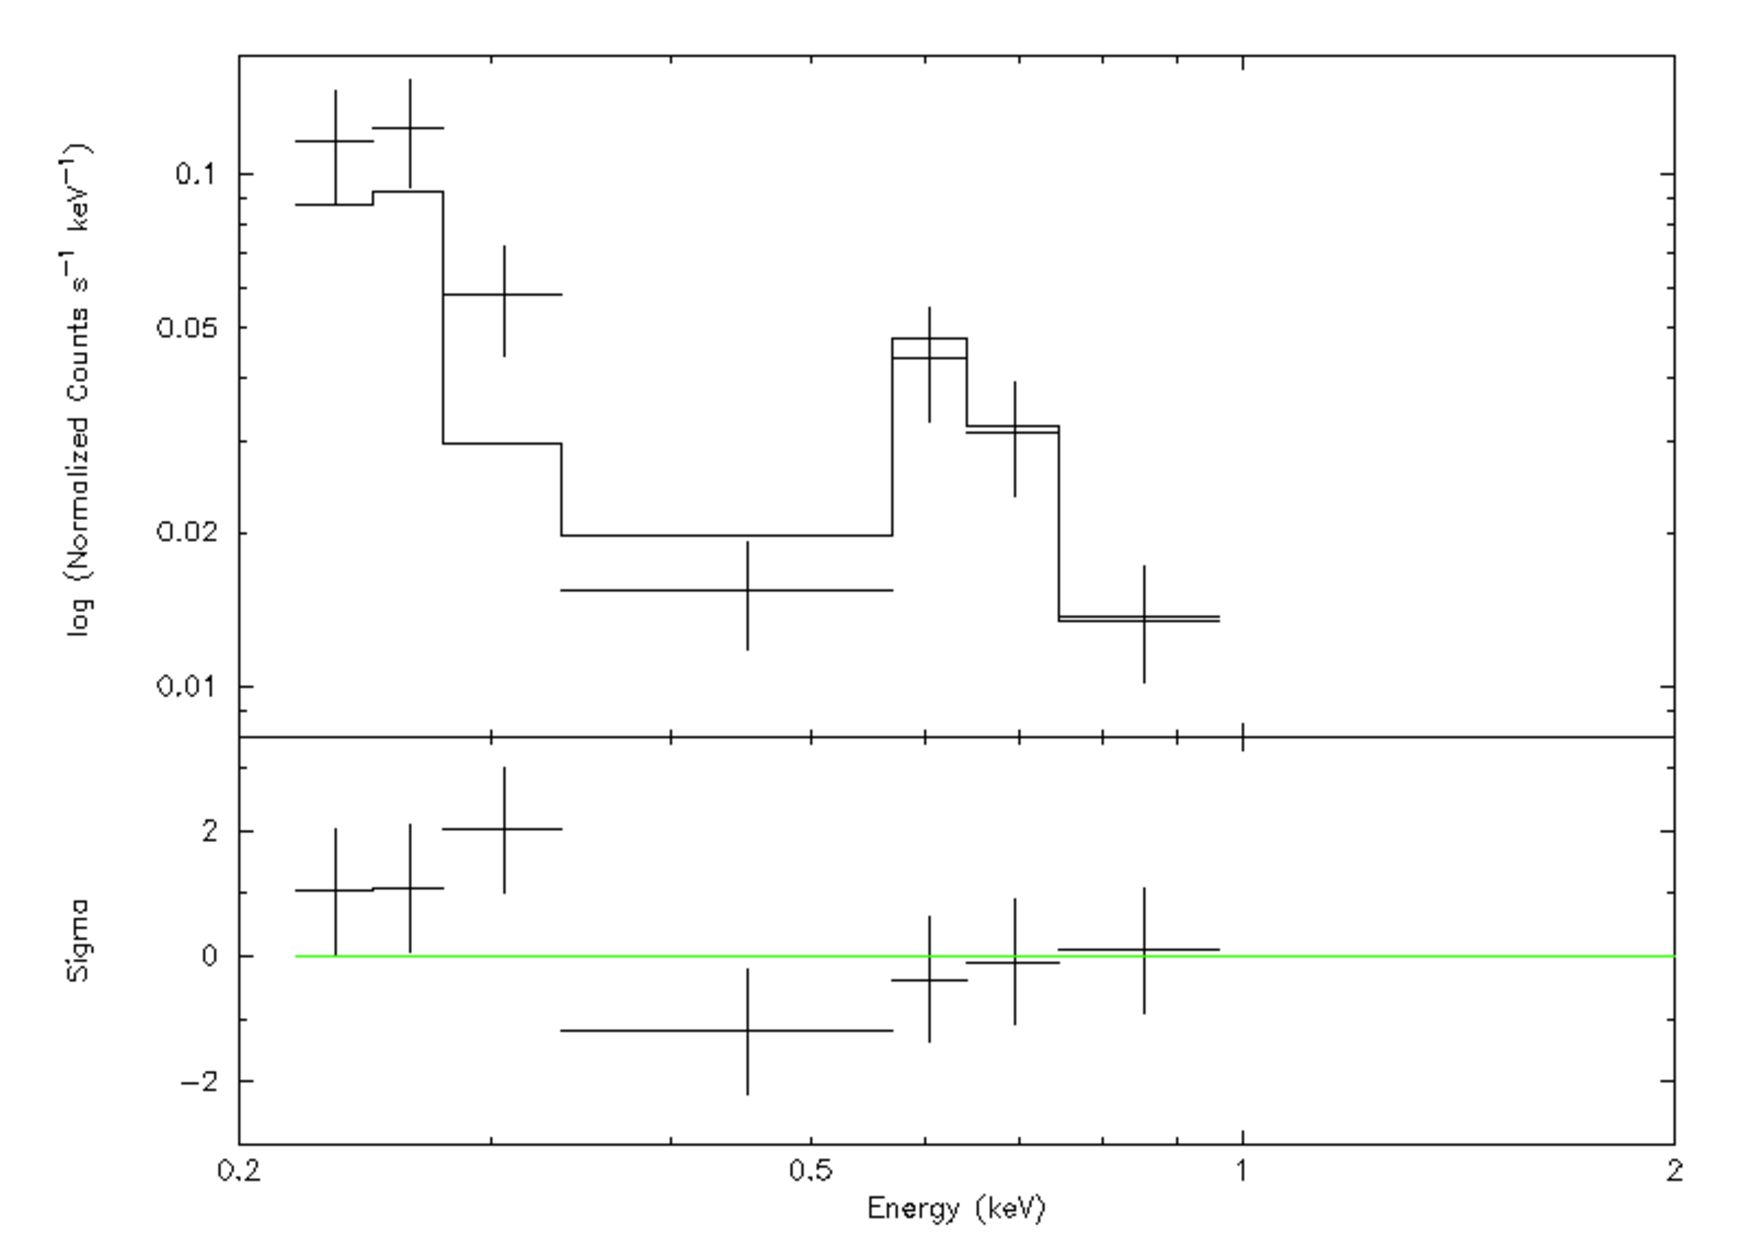
\includegraphics[height = 0.23\paperheight,width=0.9\textwidth]{Figures/3-Xray_age/spec_40eria}
	\caption{40 Eri A}
\end{subfigure}
\begin{subfigure}{\textwidth}
	\centering
	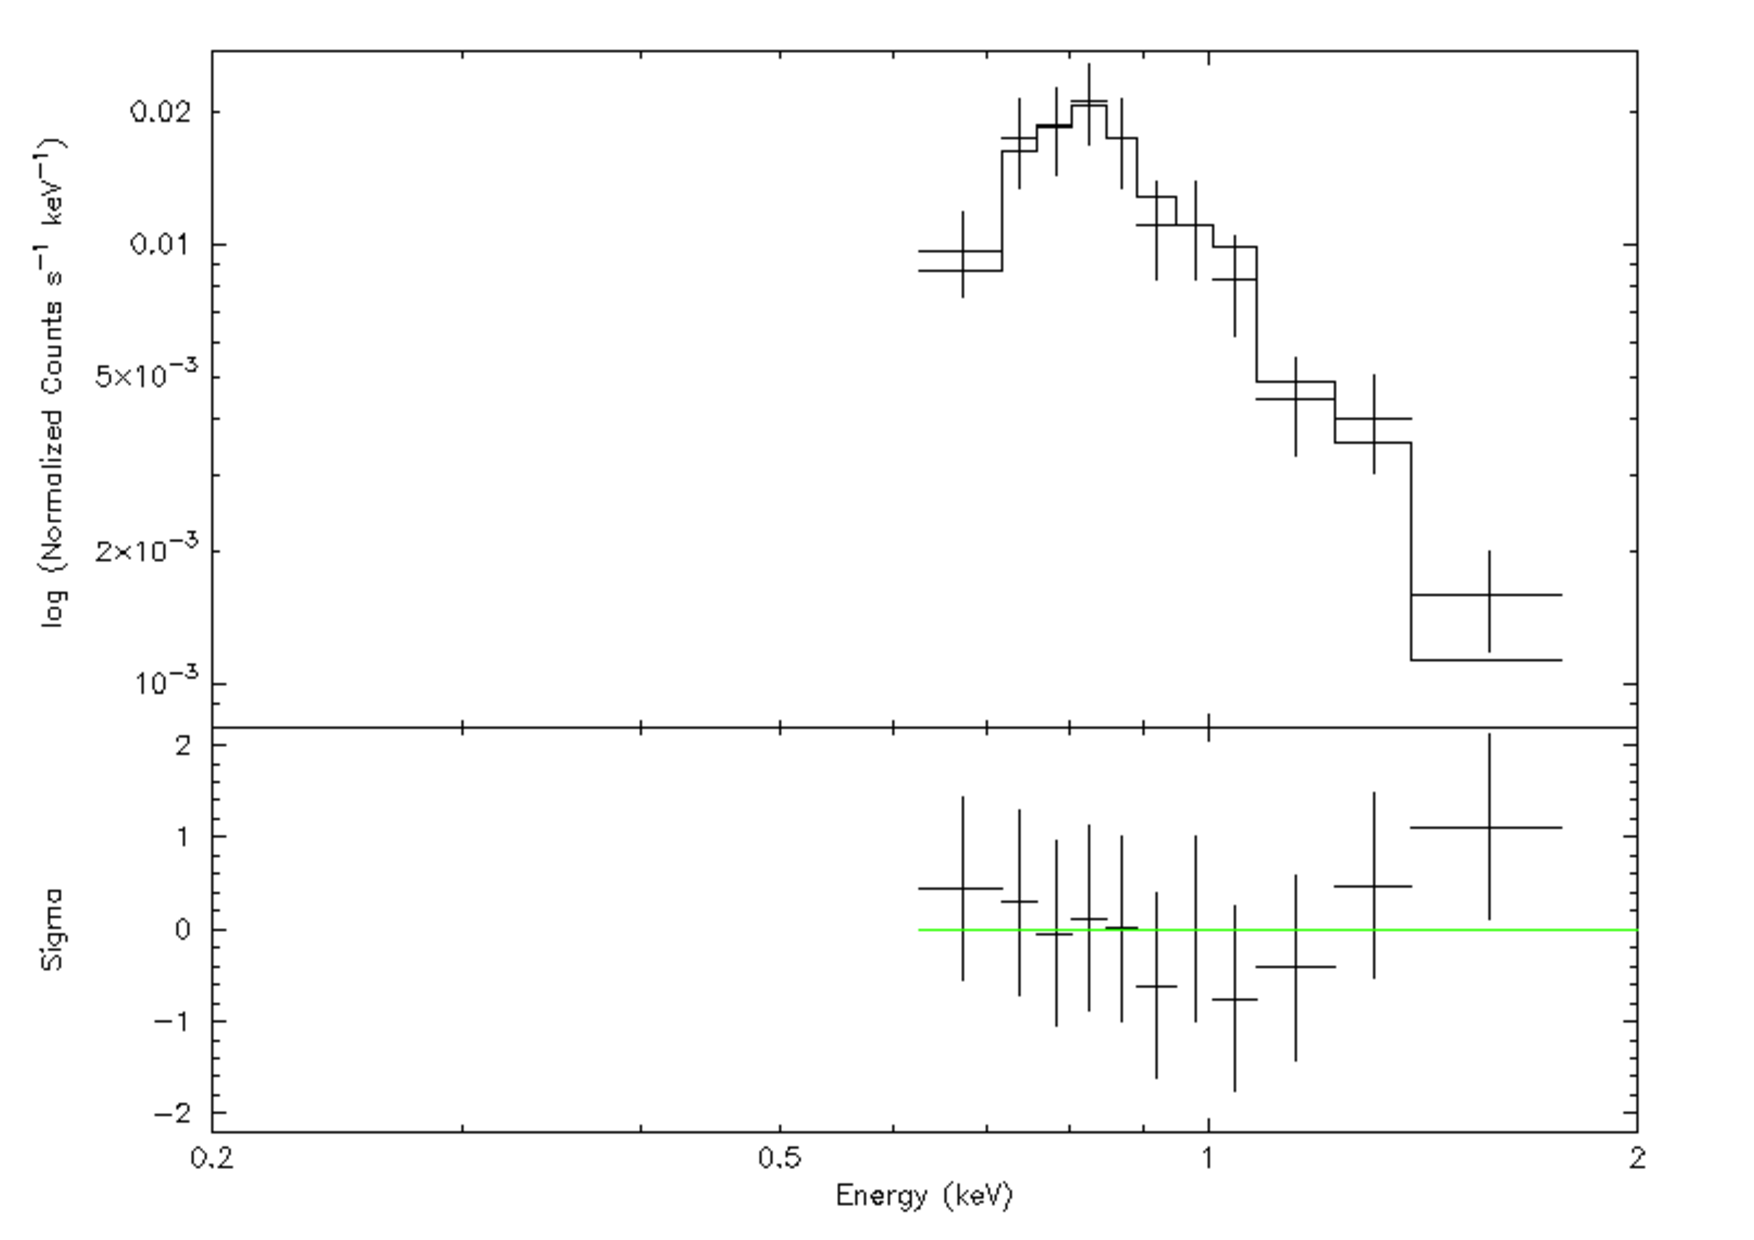
\includegraphics[height = 0.23\paperheight,width=0.9\textwidth]{Figures/3-Xray_age/spec_cd-3710500}
	\caption{CD -3710500}
\end{subfigure}

\caption[X-ray spectra of 40 Eri A and CD -3710500]{X-ray spectra (grouped to 15 counts per bin) and best fit models of two X-ray sources. The top region of each subplot shows the number of counts per second per keV as a function of energy. The bottom region of each subplot shows the sigma value for the best fit model as a function of energy. CD -3710500 was observed with a front-illuminated \textit{Chandra} CCD and therefore only has spectral data above 0.6 keV.}
\label{App_A_40EriA_CD3710500}
\end{figure}

%Second Figure
\begin{figure*}
\begin{subfigure}{\textwidth}
	\centering
	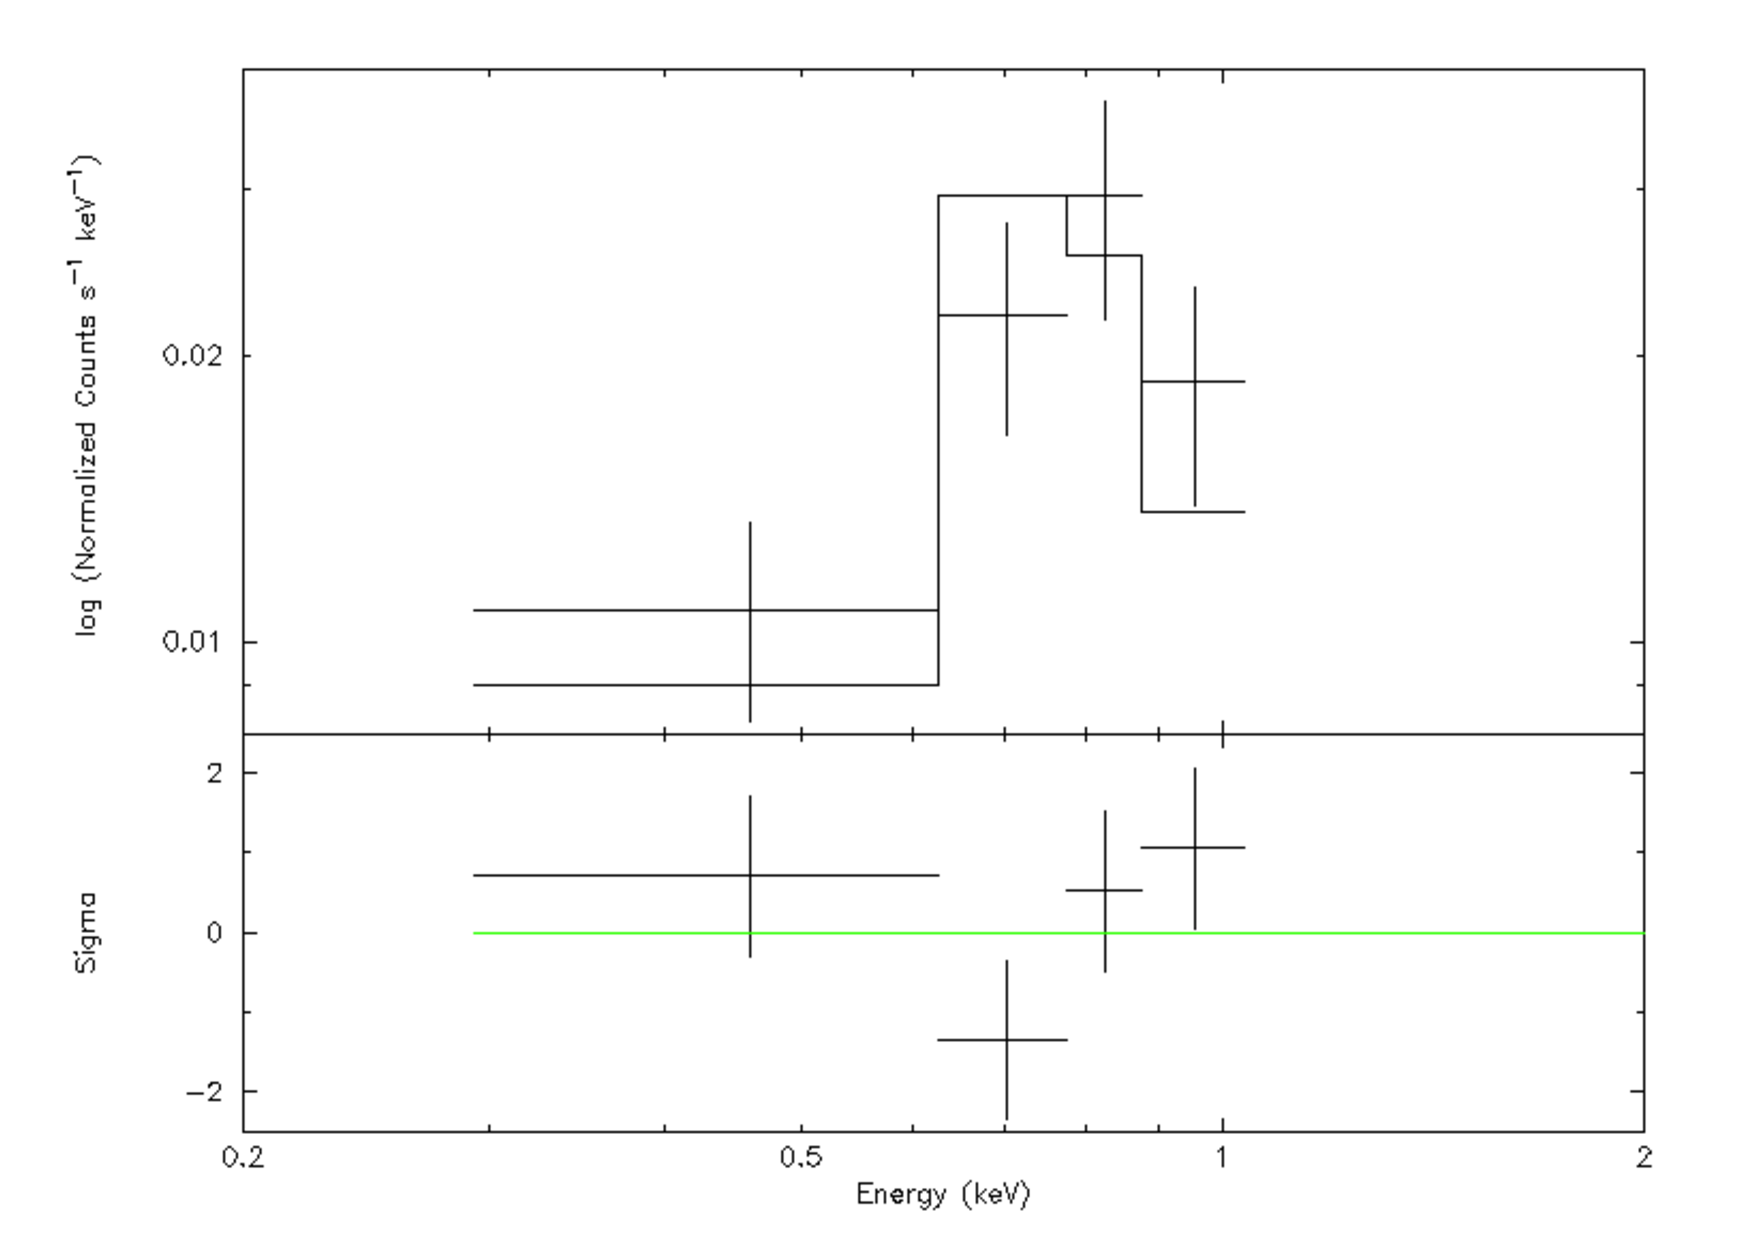
\includegraphics[height = 0.25\paperheight,width=\textwidth]{Figures/3-Xray_age/spec_gj176}
	\caption{GJ 176}
\end{subfigure}
\begin{subfigure}{\textwidth}
	\centering
	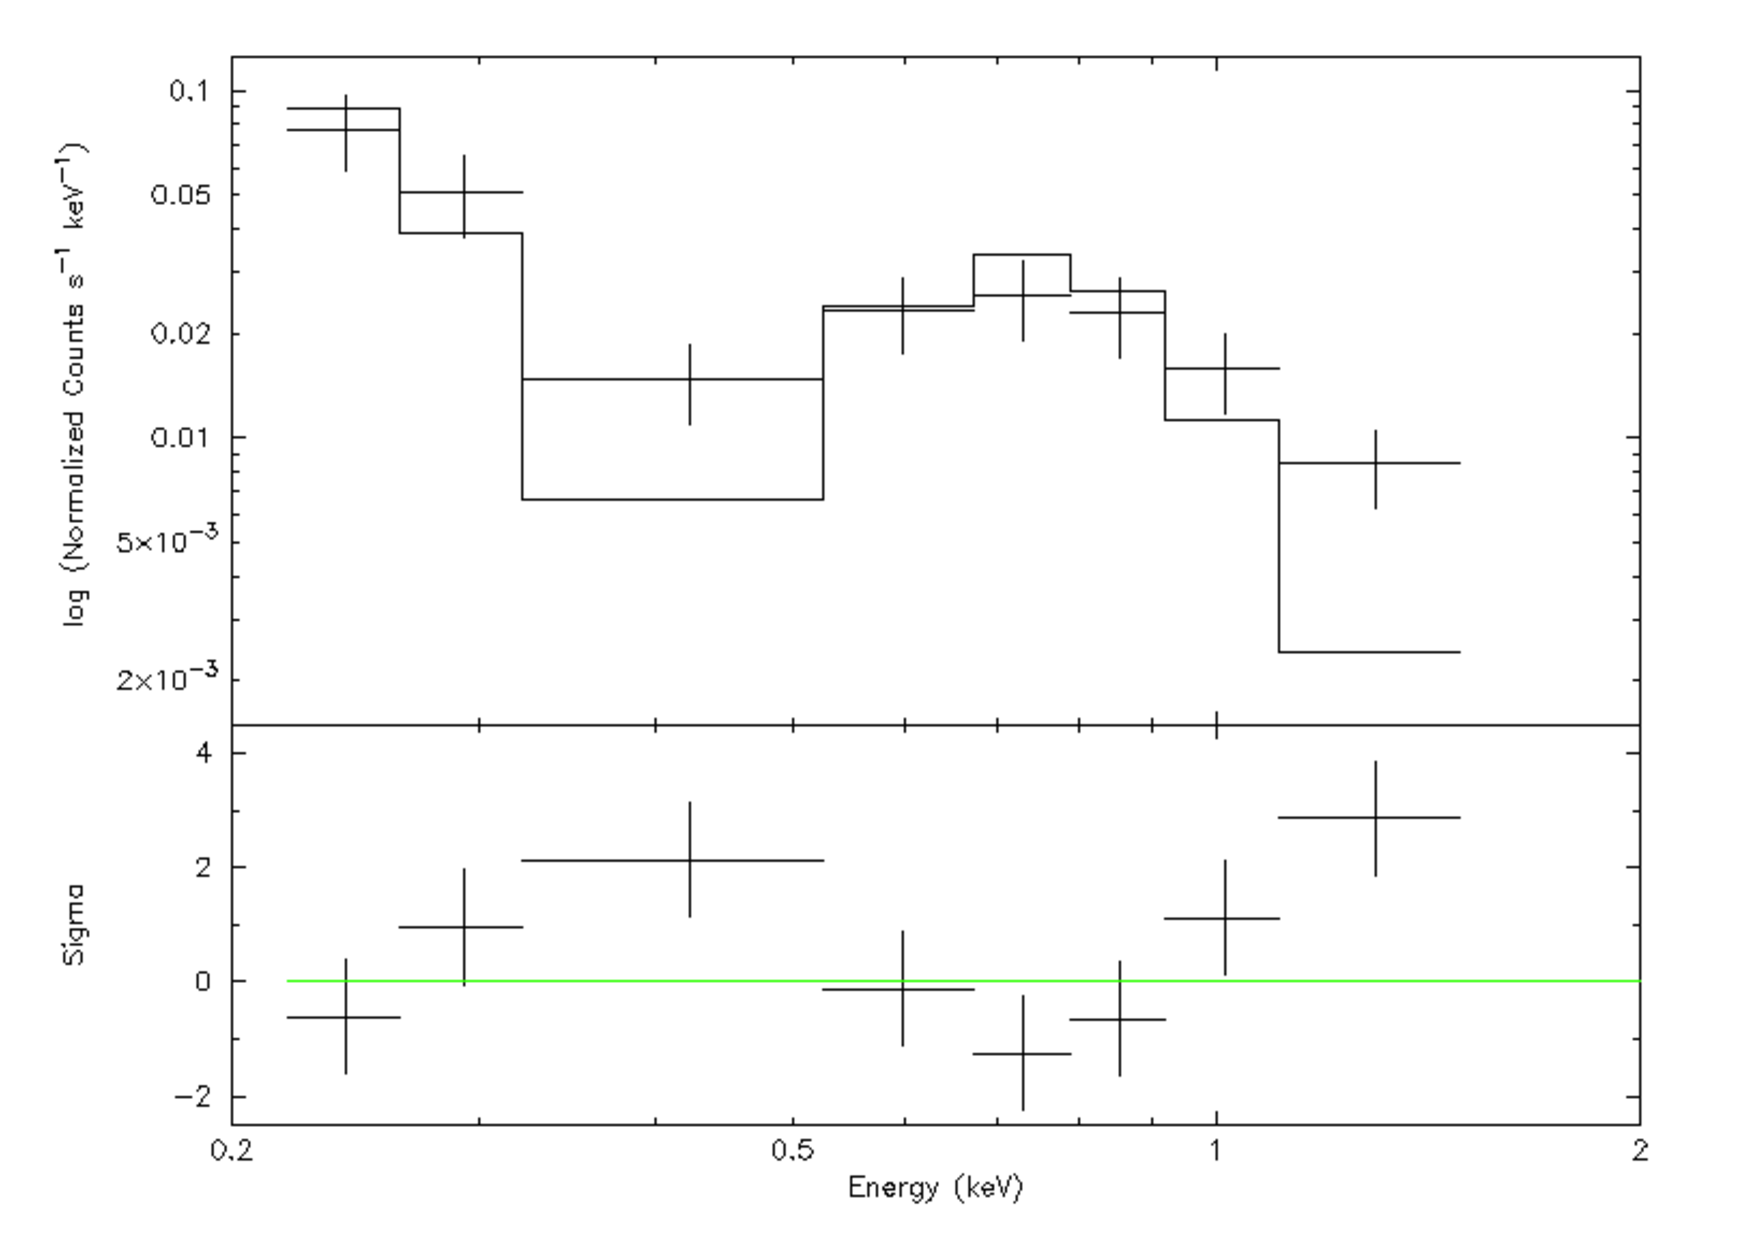
\includegraphics[height = 0.25\paperheight,width=\textwidth]{Figures/3-Xray_age/spec_gj191}
	\caption{GJ 191}
\end{subfigure}

\caption[X-ray spectra of GJ 176 and GJ 191]{X-ray spectra (grouped to 15 counts per bin) and best fit models of two X-ray sources. The top region of each subplot shows the number of counts per second per keV as a function of energy. The bottom region of each subplot shows the sigma value for the best fit model as a function of energy.}
\label{App_A_GJ176_GJ191}
\end{figure*}


%Third Figure
\begin{figure*}
\begin{subfigure}{\textwidth}
	\centering
	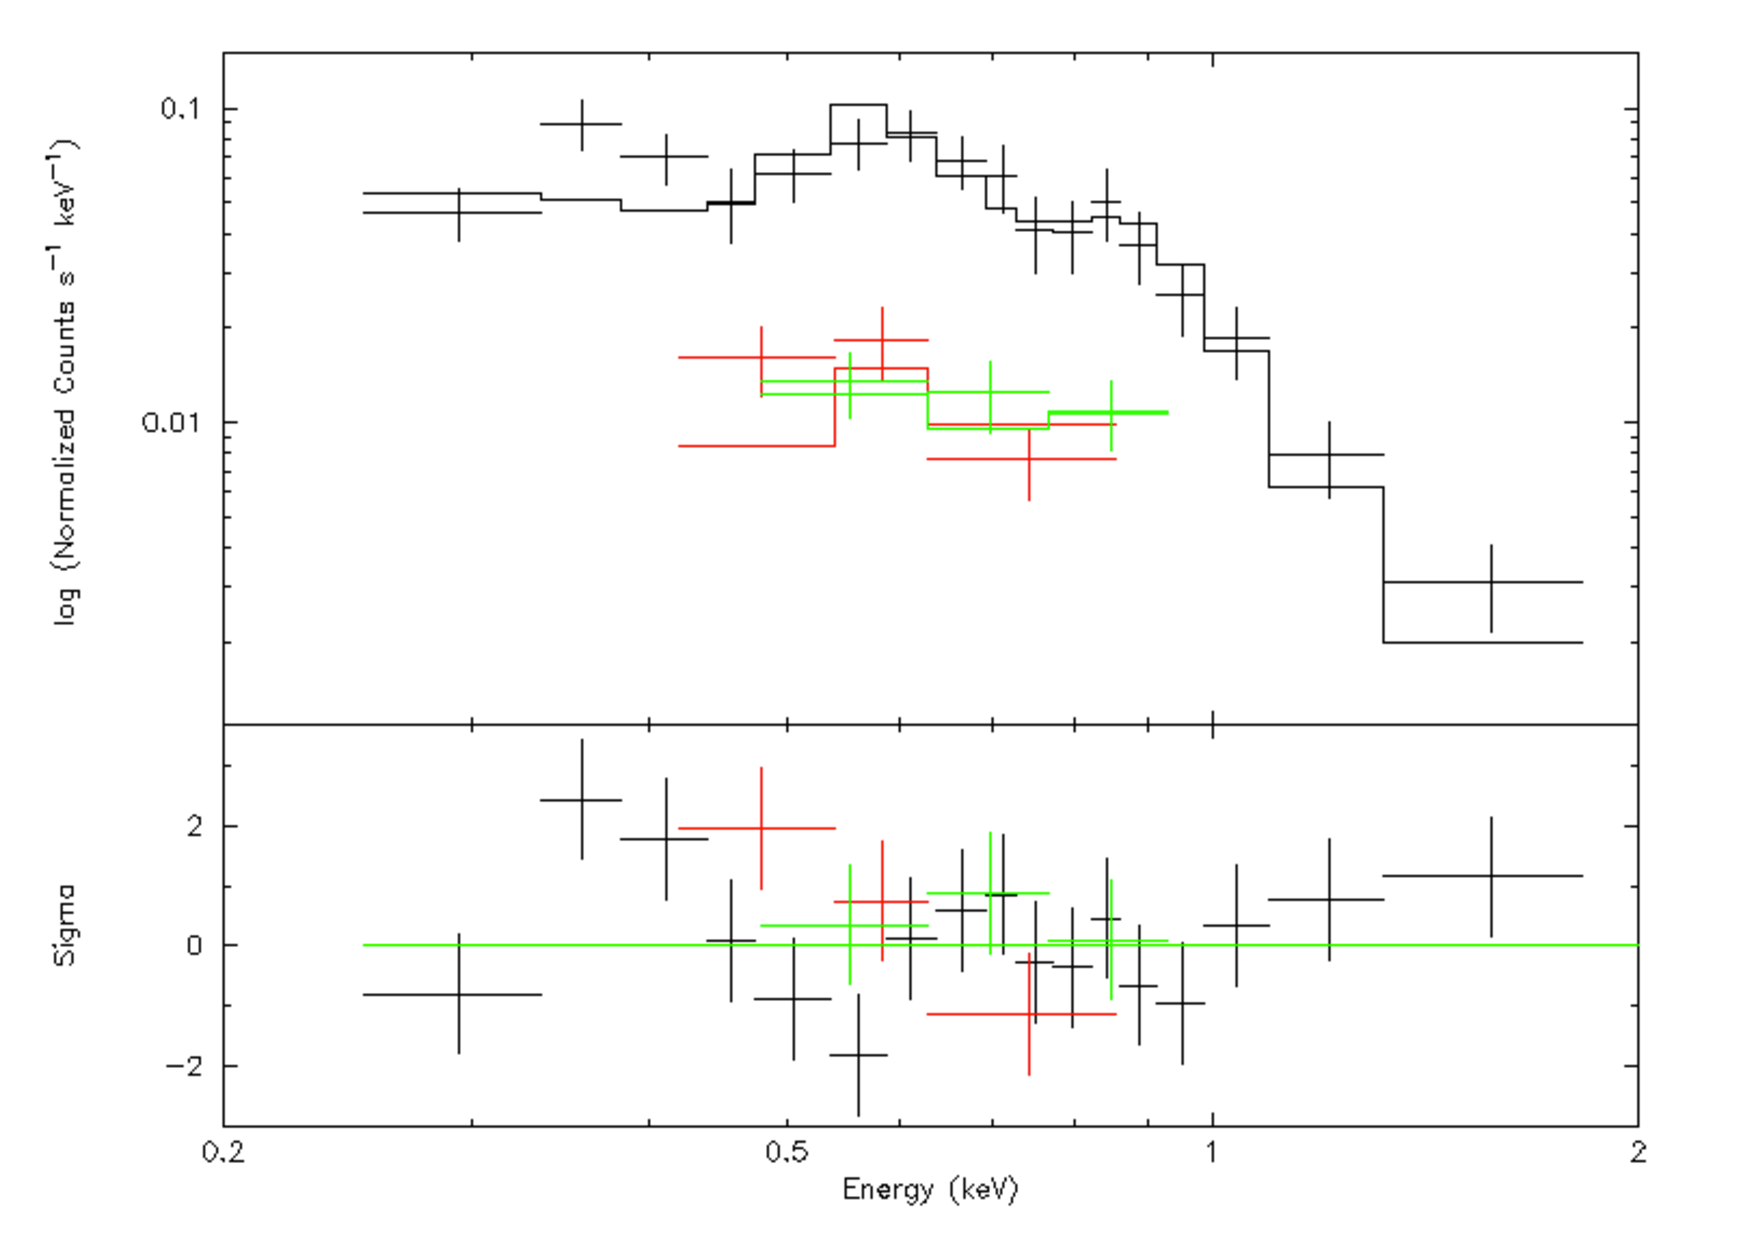
\includegraphics[height = 0.25\paperheight,width=\textwidth]{Figures/3-Xray_age/spec_hr7703}
	\caption{HR 7703}
\end{subfigure}
\begin{subfigure}{\textwidth}
	\centering
	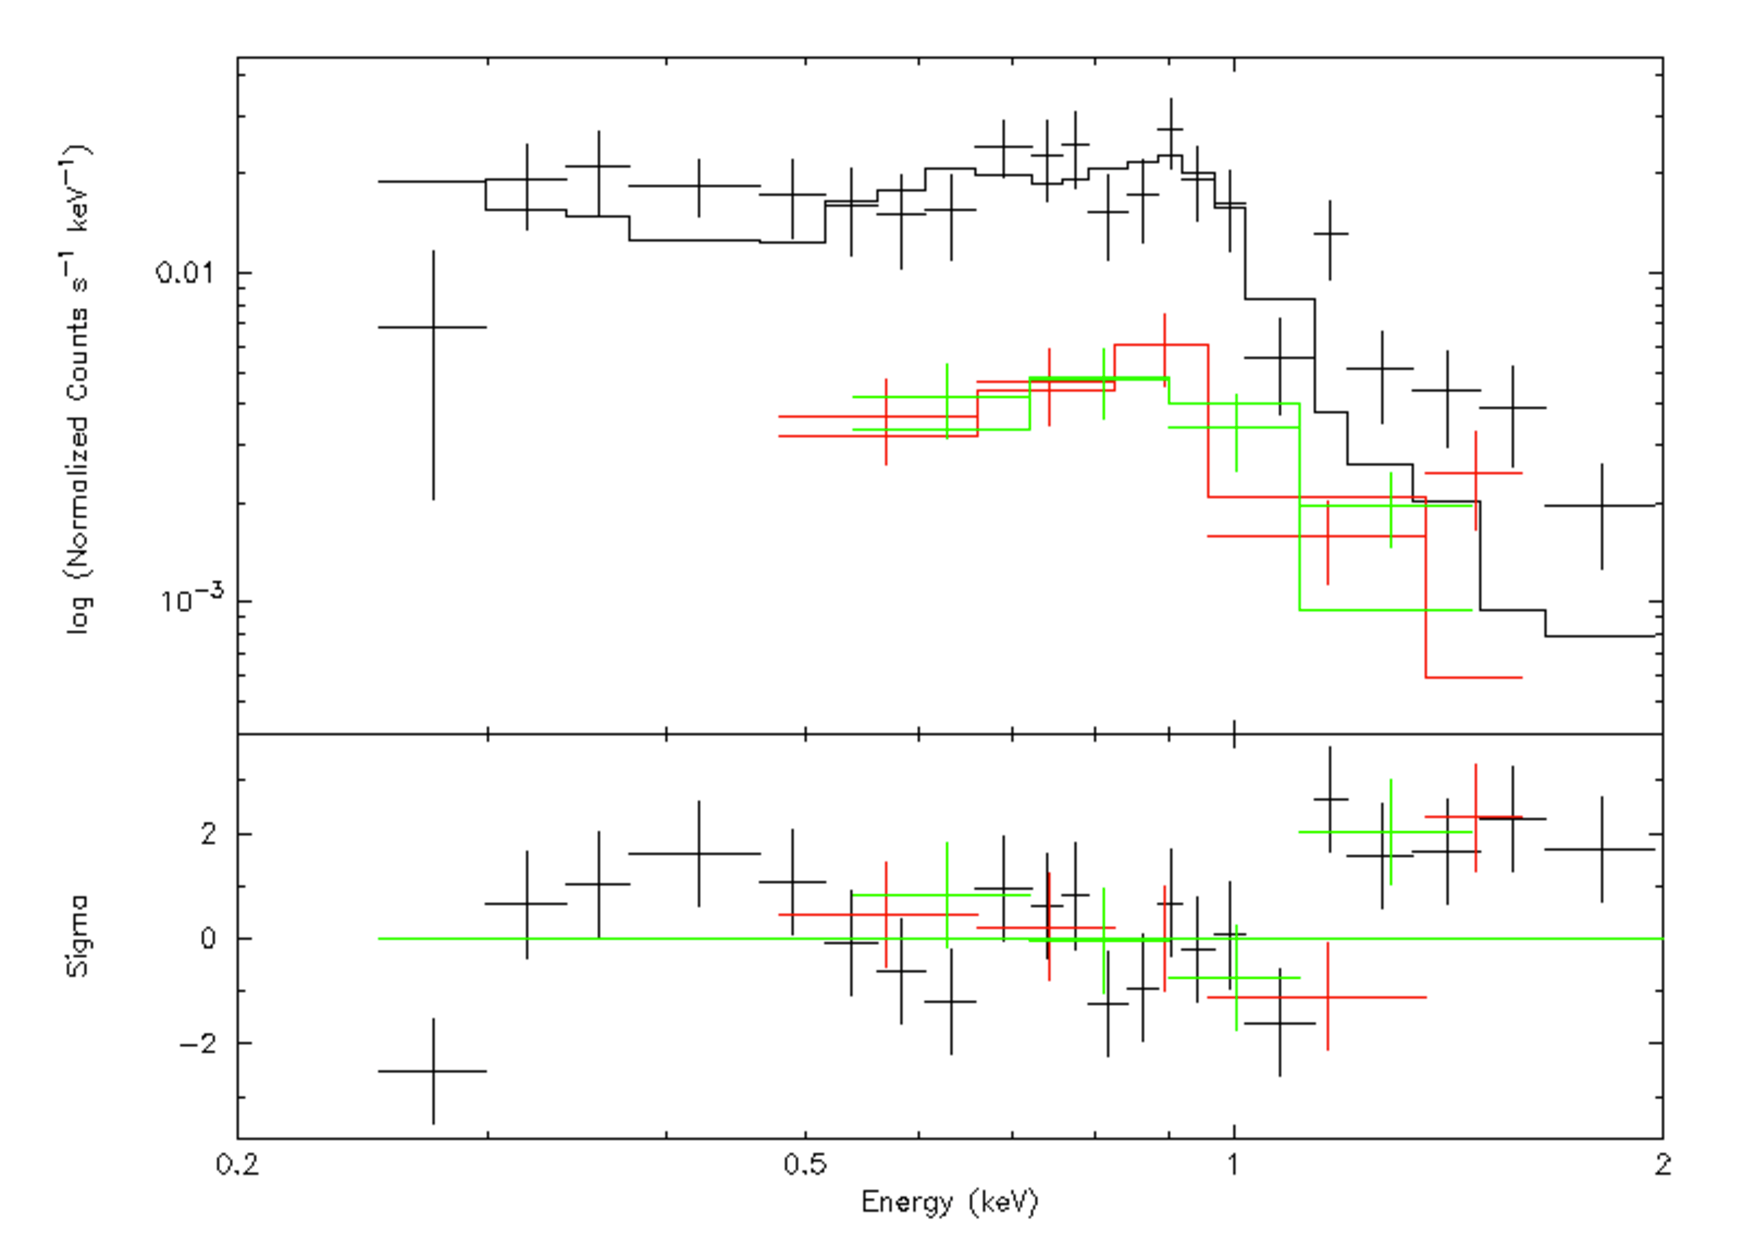
\includegraphics[height = 0.25\paperheight,width=\textwidth]{Figures/3-Xray_age/spec_kic7529180}
	\caption{KIC 7529180}
\end{subfigure}

\caption[X-ray spectra of HR 7703 and KIC 7529180]{X-ray spectra (grouped to 15 counts per bin) and best fit models of two X-ray sources. The top region of each subplot shows the number of counts per second per keV as a function of energy. The bottom region of each subplot shows the sigma value for the best fit model as a function of energy. Different colours indicate spectra from different detectors which are fitted simultaneously to ensure a more accurate fit.}
\label{App_A_HR7703_KIC7529180}
\end{figure*}

%Fourth Figure
\begin{figure*}
\begin{subfigure}{\textwidth}
	\centering
	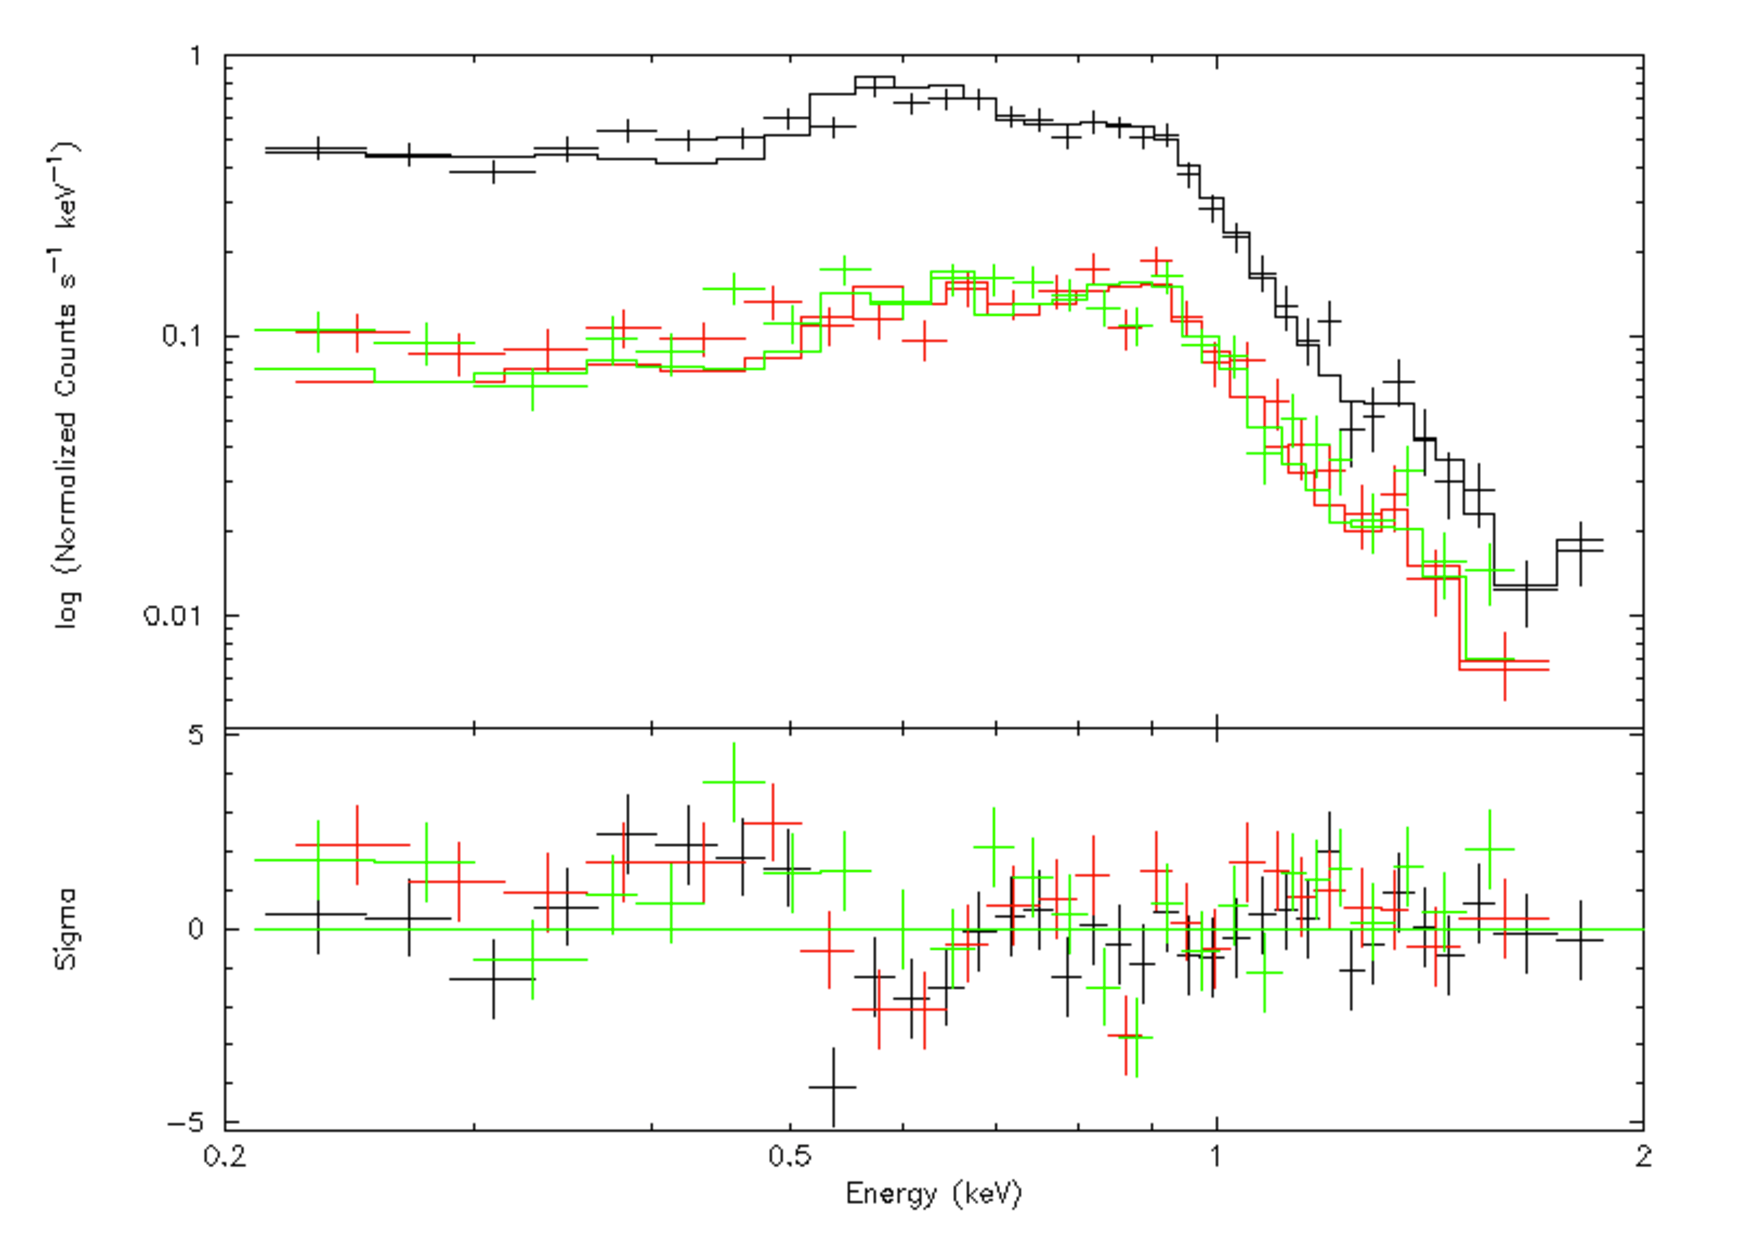
\includegraphics[height = 0.25\paperheight,width=\textwidth]{Figures/3-Xray_age/spec_61cyga}
	\caption{61 Cyg A}
\end{subfigure}
\begin{subfigure}{\textwidth}
\centering
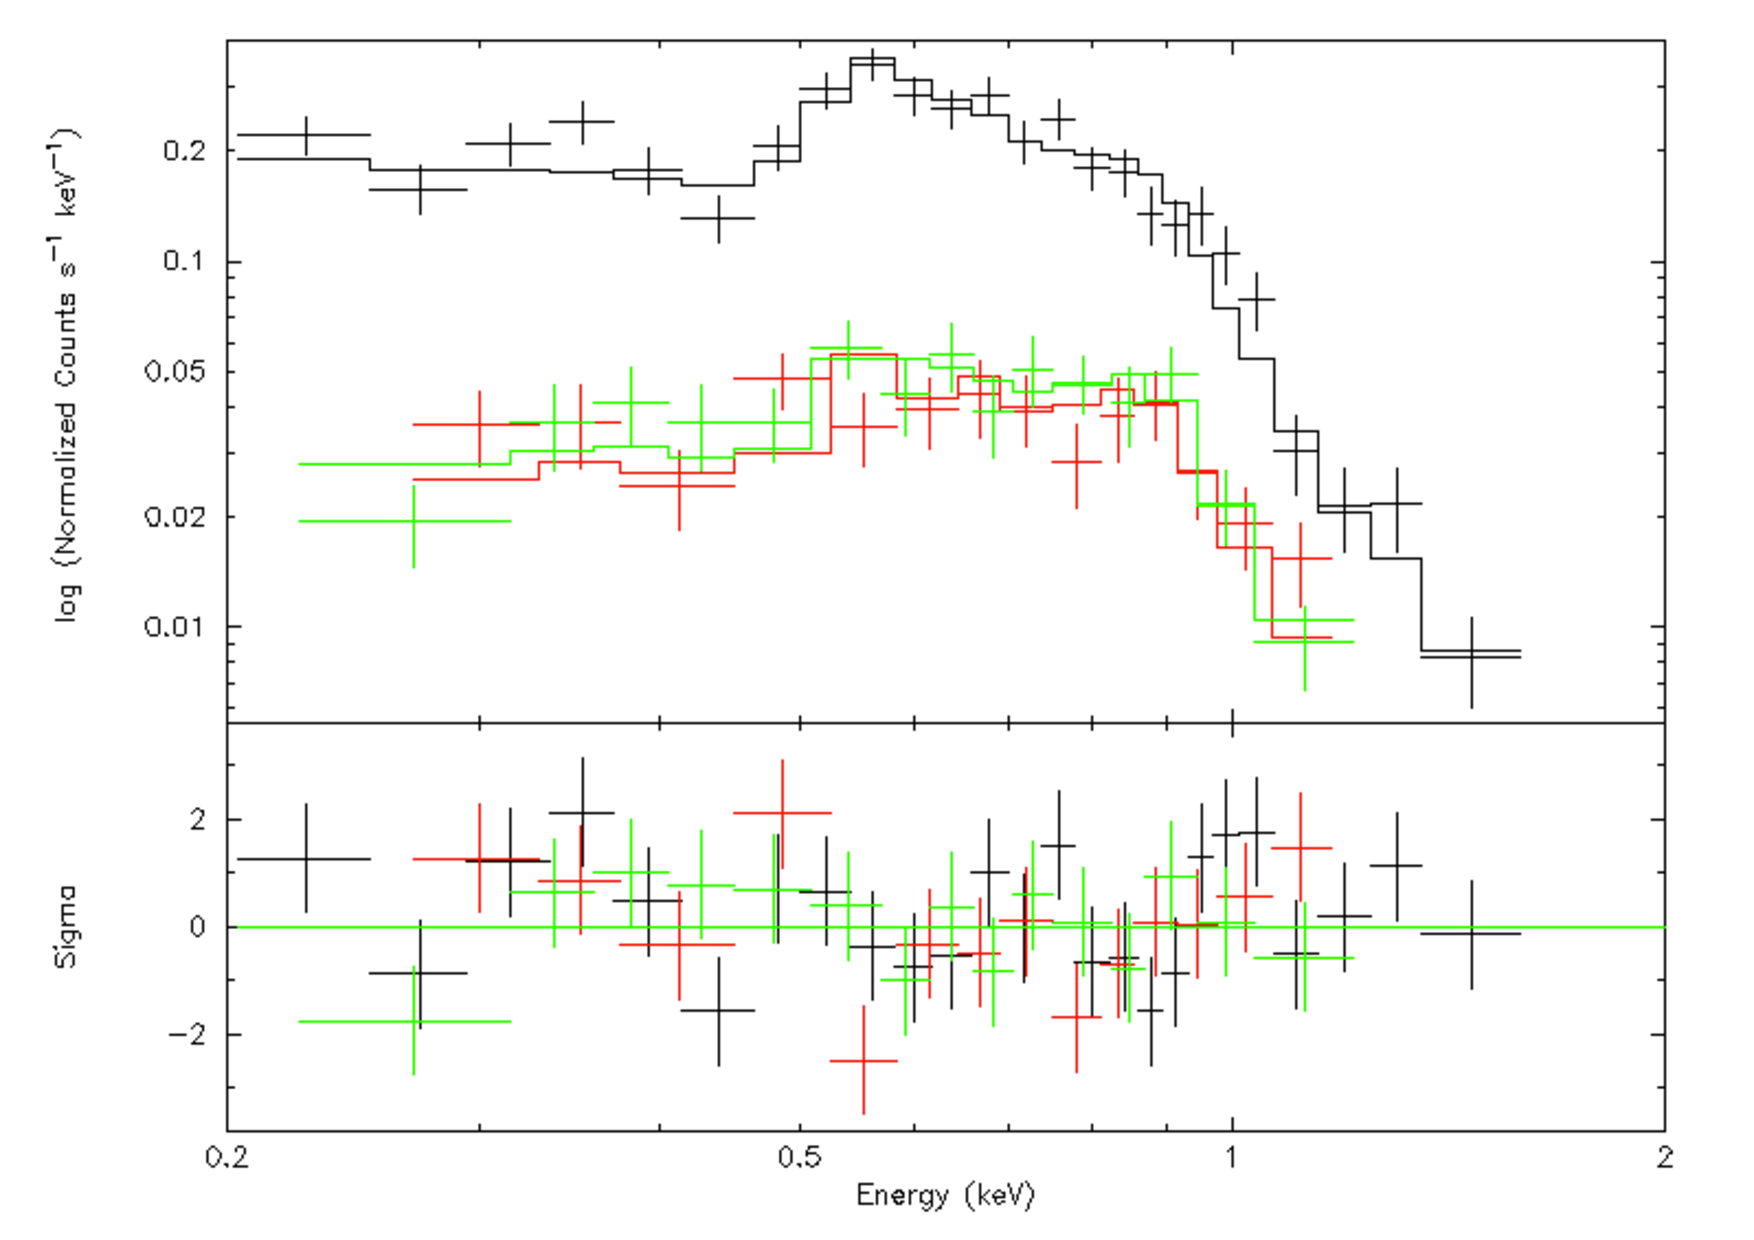
\includegraphics[height =        0.25\paperheight,width=\textwidth]{Figures/3-Xray_age/spec_61cygb}
\caption{61 Cyg B}
\end{subfigure}
\par\bigskip

\caption[X-ray spectra of 61 Cyg A and B]{X-ray spectra (grouped to 15 counts per bin) and best fit models for one exemplary observation of 61 Cyg A and B, respectively. These sources were detected to at least three sigma and contained over a hundred counts in the source region. The top region of each subplot shows the number of counts per second per keV as a function of energy. The bottom region of each subplot shows the sigma value for the best fit model as a function of energy. Different colours indicate spectra from different detectors which are fitted simultaneously to ensure a more accurate fit.}
\label{App_A_61Cyg}
\end{figure*}
\clearpage

%Appendix B
\chapter{X-ray luminosity and age results}
\label{App_lx_results}

\begin{small}
\begin{landscape}
\begin{longtable}{lccccccc}

\caption[Full X-ray luminosity results]{Stellar ages and X-ray luminosities for stellar sample considered in Chapter \ref{Chapter3}.\\
\textbf{References}: (1) \citet{Silva_Aguirre_etal_2017}; (2) this work, age recalculated with BASTA algorithm \citep{Silva_Aguirre_etal_2015} using values from \citet{Chaplin_etal_2014} and  \citet{Buchhave_Latham_2015}; (3) \citet{Silva_Aguirre_etal_2015}; (4) this work, see Section \ref{Section_sample_selection}; (5) \citet{Kervella_etal_2008}; (6) \citet{Feltzing_Holmberg_2000}; (7) \citet{Anglada_Escude_etal_2014}; (8) \citet{DeWarf_etal_2010}; (9) \citet{Miglio_Montalban_2005}; (10) \citet{Bahcall_etal_1995}}\\

\hline
Name of Star & Age & log($L_{x}$) & log($L_{x}/R_{\odot}^{2}$) & Spectral Type & Age Determination &Age Ref. \\
/ White Dwarf&/ Gyr&log(ergs s$^{-1}$)&log(ergs s$^{-1}$ $R_{\odot}^{-2}$)&&&\\
\hline
\endfirsthead

\hline
Name of Star & Age / Gyr & log($L_{x}$) & log($L_{x}/R_{\odot}^{2}$) & Spectral Type & Age Determination &Age Ref. \\
/ White Dwarf&&log(ergs s$^{-1}$)&log(ergs s$^{-1}$ $R_{\odot}^{-2}$)&&&\\
\hline
\endhead

\hline
\endfoot
 
\hline
\endlastfoot

16 Cyg A & $6.67^{0.81}_{0.77}$  & $26.89^{0.10}_{0.10}$ & $26.71^{0.10}_{0.10}$ & G1.5Vb & Asteroseismology & 1  \\
16 Cyg B & $7.39^{0.89}_{0.91}$ & $<25.85$   & $<25.77$ & G3V & Asteroseismology  & 1  \\
40 Eri A / 40 Eri B & $3.70^{3.57}_{1.34}$ & $26.81^{0.10}_{0.10}$ & $26.97^{0.10}_{0.10}$ & K0.5V & White Dwarf & 4 \\
61 Cyg A \footnote{X-ray luminosity adopted from \citet{Robrade_etal_2012}} & $6.00^{1.00}_{1.00}$ & $27.08^{0.23}_{0.23}$ & $27.43^{0.23}_{0.23}$ & K5Ve & Isochrone Fitting & 5 \\
61 Cyg B \footnote{X-ray luminosity adopted from \citet{Robrade_etal_2012}} & $6.00^{1.00}_{1.00}$ & $26.88^{0.10}_{0.10}$ & $27.33^{0.10}_{0.10}$ & K7V & Isochrone Fitting & 5 \\
CD -3710500 / L481-60 & $1.77^{0.65}_{0.27}$ & $28.18^{0.10}_{0.10}$ & $28.22^{0.10}_{0.10}$ & G7IV & White Dwarf & 4 \\
GJ 176 & $2.00^{0.80}_{0.80}$ & $27.03^{0.10}_{0.10}$ & $27.80^{0.10}_{0.10}$ & M2.5V & Member of HR 1614 & 6 \\
GJ 191 & $11.00^{1.00}_{1.00}$ & $26.41^{0.10}_{0.10}$ & $27.02^{0.10}_{0.10}$ & sdM1.0 & Galactic Halo population & 7 \\
HR 7703 & $10.00^{2.00}_{2.00}$ & $26.80^{0.10}_{0.10}$ & $27.04^{0.10}_{0.10}$ & K2.5V & Old disk star & 8 \\
KIC 10016239 & $2.47^{0.67}_{0.61}$ & $27.91^{0.10}_{0.10}$ & $27.71^{0.10}_{0.10}$ & F6IV & Asteroseismology & 2 \\
KIC 12011630 & $8.48^{1.53}_{1.42}$ & $<30.06$ & $<30.05$ & G1.5V & Asteroseismology & 2 \\
KIC 3123191 & $4.26^{0.80}_{0.75}$ & $<29.12$ & $<28.84$ & F4.5V & Asteroseismology & 2 \\
KIC 5309966 & $3.51^{1.23}_{0.42}$ & $<29.44$ & $<29.02$ & F6V & Asteroseismology & 2 \\
KIC 6116048 & $9.58^{2.16}_{1.90}$ & $<26.89$ & $<26.74$ & F9IV-V & Asteroseismology & 1 \\
KIC 6603624 & $7.82^{0.94}_{0.86}$ & $<27.08$ & $<26.96$ & G8IV-V & Asteroseismology & 1 \\
KIC 7529180 & $1.93^{0.35}_{0.30}$ & $28.98^{0.10}_{0.10}$ & $28.66^{0.10}_{0.10}$ & F5IV-V & Asteroseismology & 2 \\
KIC 8292840 & $3.85^{0.81}_{0.75}$ & $<28.14$ & $<27.88$ & F7V & Asteroseismology & 3 \\
KIC 9025370 & $6.55^{1.26}_{1.13}$ & $<27.24$ & $<27.23$ & F8 & Asteroseismology & 1 \\
KIC 9410862 & $6.93^{1.49}_{1.33}$ & $<27.98$ & $<27.86$ & F7V & Asteroseismology & 1 \\
KIC 9955598 & $6.98^{0.40}_{0.50}$ & $26.90^{0.10}_{0.10}$ & $27.01^{0.10}_{0.10}$ & K0V & Asteroseismology & 3 \\
NLTT 7887 / NLTT 7890 & $4.97^{8.80}_{3.00}$ & $<26.92$ & $<27.13$ & K2 & White Dwarf & 4 \\
Proxima Centauri  \footnote{X-ray luminosity taken from \citet{Fuhrmeister_etal_2011}} & $6.13^{0.55}_{0.55}$ & $26.69^{0.10}_{0.10}$ & $28.23^{0.10}_{0.10}$ & M5.5Ve & Asteroseismology & 9 \\
Alpha Centauri B \footnote{X-ray luminosity adopted from \citet{Robrade_etal_2012}} & $6.13^{0.55}_{0.55}$ & $27.06^{0.36}_{0.36}$ & $27.19^{0.36}_{0.36}$ & K1V & Asteroseismology & 9 \\
Sun \footnote{X-ray luminosity adapted from model values given in \citet{Peres_etal_2000}} & $4.57^{0.02}_{0.02}$ & $26.77^{0.72}_{0.72}$ & $26.77^{0.72}_{0.72}$ & G2V & Isotopic Dating & 10 \\
\hline  
\end{longtable}
\end{landscape}
\end{small}

\clearpage

%Appendix C
\chapter{Stellar properties of X-ray sample}
\label{App_Xray_sample_stellar_properties}

\begin{small}
\begin{table}[h!]
\centering
\resizebox{0.9\textwidth}{!}{
	\begin{tabular}[h]{l c c c c l}
		\hline
		Name of Star / White Dwarf & Radius / $R_{\odot}$ & $T_{eff}$ / K & $V_{mag}$ & Distance / pc & References\\
		\hline 
		16 Cyg A & 1.22 & 5825 & 5.95 & 21.29 & 1,6,8,10 \\
		16 Cyg B & 1.10 & 5720 & 6.20 & 21.22 & 1,6,8,10  \\
		40 Eri A / 40 Eri B & 0.83  & 5225 & 4.43 & 4.98 & 5,6,8,9 \\
		61 Cyg A & 0.67 & 4450 & 5.21 & 3.49 & 4,6,8,9 \\
		61 Cyg B & 0.60 & 4050 & 6.03 & 3.50 & 4,6,8,9 \\
		CD -3710500 / L481-60 & 0.96 & 5530 & 6.01 & 15.25 & 5,6,8,10 \\
		GJ 176 & 0.41 & 3475 & 9.95 & 9.27 & 5,6,8,9 \\
		GJ 191  & 0.49 & 3680 & 8.85 & 3.91 & 5,6,8,9 \\
		HR 7703 & 0.77 & 4940 & 5.32 & 6.02 & 5,6,8,9 \\
		KIC 10016239 & 1.26 & 6482 & 9.81 & 175.93 & 3,7,8,10 \\
		KIC 12011630 & 1.01 & 5817 & 10.27 & 114.40 & 3,7,8,11 \\
		KIC 3123191 & 1.37 & 6568 & 9.90 & 167.67 & 3,7,8,10 \\
		KIC 5309966 & 1.62 & 6356 & 10.62 & 288.60 & 3,7,8,10 \\
		KIC 6116048 & 1.19 & 6072 & 8.47 & 75.15 & 1,7,8,10 \\
		KIC 6603624 & 1.15 & 5612 & 9.19 & 83.56 & 1,7,8,10 \\
		KIC 7529180 & 1.45 & 6682 & 8.49 & 108.53 & 3,7,8,10 \\
		KIC 8292840 & 1.35 & 6239 & 10.51 & 250.69 & 2,2,8,9 \\
		KIC 9025370 & 1.00 & 5659 & 8.95 & 87.42 & 1,7,8,10 \\
		KIC 9410862 & 1.16 & 6230 & 10.78 & 202.27 & 1,7,8,10 \\
		KIC 9955598 & 0.88 & 5434 & 9.64 & 69.39 & 2,7,8,10 \\
		NLTT 7887 / NLTT 7890 & 0.78 & 5040 & 9.84 & 41.16 & 5,6,8,10 \\
		Proxima Centauri & 0.17 & 2925 & 11.13 & 1.30 & 5,6,8,9 \\
		Alpha Centauri B & 0.86 & 5316 & 1.33 & 1.35 & 12,12,8,12 \\
		Sun  & 1.00 & 5777 & -26.74 & 1 AU & 13 \\    
		\hline 
	\end{tabular}}
	
	\caption[Stellar properties of X-ray luminosity sample]{Stellar properties for the sample of stars considered in Chapter \ref{Chapter3}.\textbf{References}: (1) \citet{Silva_Aguirre_etal_2017}; (2) \citet{Silva_Aguirre_etal_2015}; (3) this work, radius recalculated with BASTA algorithm \citep{Silva_Aguirre_etal_2015} using values from \citet{Chaplin_etal_2014} and  \citet{Buchhave_Latham_2015}; (4) \citet{Kervella_etal_2008}; (5) Radius calculated from $T_{eff}$ and absolute brightness; (6) $T_{eff}$ estimated from Spectral Type using Table 5 from \citet{Pecaut_Mamajek_2013}; (7) \citet{Chaplin_etal_2014}
	(8) $V_{mag}$ from SIMBAD; (9) Parallax from SIMBAD; (10) Parallax from \textit{Gaia} DR1 \citep{Gaia_Collaboration_2016_DR1}; (11) Distance from Barnes-Evans method (see Section \ref{Section_Xray_distances_and_spectype} for details); (12) \citet{DeWarf_etal_2010}}
\end{table}

\end{small}

\clearpage

%Appendix D
\chapter{Stars used to calibrate to \texorpdfstring{\Smw}{Smw} index}
\label{App_calibrator_stars_Smw}

\begin{small}
%ESPADONS TABLE
\begin{longtable}{llccc}
\caption[\esp calibrator stars for \Smw relationship]{List of calibrator stars \citep{Duncan_etal_1991} used to calibrate the relationship between the S index calculated from \esp spectra and \Smw. Spectral types and $B-V$ taken from SIMBAD \citep{Wenger_etal_2000}.}\\

\hline
Star Name         & Spectral Type & $B-V$  & Average \Smw & \esp S Index \\
\hline
\endfirsthead

\hline
Star Name         & Spectral Type & $B-V$  & Average \Smw & \esp S Index \\
\hline
\endhead

\hline
\endfoot
 
\hline
\endlastfoot

\renewcommand{\arraystretch}{1.2}

Cl Melotte 22 1613 & G0            & 0.54 & 0.3077 & $0.0119^{0.0006}_{0.0006}$\\
HD 124897          & K1.5III       & 1.23 & 0.1441 & $0.0075^{0.0001}_{0.0001}$\\
HD 144579          & G8V           & 0.73 & 0.1628 & $0.0081^{0.0005}_{0.0005}$\\
HD 159181          & G2Ib-IIa      & 0.98 & 0.3019 & $0.0167^{0.0002}_{0.0002}$\\
HD 171635          & F7Ib          & 0.62 & 0.0499 & $0.0017^{0.00002}_{0.00002}$\\
HD 177241          & G9IIIb        & 1.00 & 0.1057 & $0.0053^{0.0001}_{0.0001}$\\
HD 179958          & G2V           & 0.65 & 0.1571 & $0.0068^{0.0002}_{0.0002}$\\
HD 182572          & G7IV          & 0.77 & 0.1543 & $0.0071^{0.0002}_{0.0002}$\\
HD 185351          & G8.5IIIb      & 0.94 & 0.1946 & $0.0116^{0.0001}_{0.0001}$\\
HD 186408          & G1.5Vb        & 0.64 & 0.1476 & $0.0071^{0.0001}_{0.0001}$\\
HD 186427          & G3V           & 0.66 & 0.1450 & $0.0073^{0.0003}_{0.0003}$\\
HD 187691          & F8V           & 0.56 & 0.1479 & $0.0059^{0.0004}_{0.0004}$\\
HD 192876          & G3Ib          & 1.07 & 0.2510 & $0.0129^{0.0001}_{0.0001}$\\
HD 194093          & F8Ib          & 0.67 & 0.0564 & $0.0039^{0.0005}_{0.0005}$\\
HD 204867          & G0Ib          & 0.82 & 0.1617 & $0.0074^{0.0001}_{0.0001}$\\
HD 206859          & G5Ib          & 1.17 & 0.2041 & $0.0140^{0.0002}_{0.0002}$\\
HD 209750          & G2Ib          & 0.96 & 0.2081 & $0.0117^{0.0001}_{0.0001}$\\
HD 217014          & G2IV          & 0.70 & 0.1548 & $0.0068^{0.0002}_{0.0002}$\\
HD 26630           & G0Ib          & 0.96 & 0.3623 & $0.0148^{0.0001}_{0.0001}$\\
HD 31910           & G1Ib          & 0.93 & 0.2659 & $0.0124^{0.0001}_{0.0001}$\\
HD 3795            & K0V           & 0.70 & 0.1587 & $0.0069^{0.0001}_{0.0001}$\\
HD 39587           & G0V           & 0.60 & 0.3067 & $0.0173^{0.0001}_{0.0001}$\\
HD 7924            & K0.5V         & 0.85 & 0.2221 & $0.0102^{0.0001}_{0.0001}$\\
HD 89449           & F6IV-V        & 0.44 & 0.1781 & $0.0078^{0.0001}_{0.0001}$\\
HD 98736		   & G5			   & 0.84 & 0.1940 & $0.0096^{0.0001}_{0.0001}$\\
Parenago 1394	   & F8			   & 0.48 & 0.2635 & $0.0141^{0.0003}_{0.0003}$\\
\hline
\end{longtable}
\end{small}

%NARVAL TABLE
\begin{small}
\begin{longtable}{llccc}
\caption[\narval calibrator stars for \Smw relationship]{List of calibrator stars \citep{Duncan_etal_1991} used to calibrate the relationship between the S index calculated from \narval spectra and \Smw. Spectral types and $B-V$ taken from SIMBAD \citep{Wenger_etal_2000}.}\\

\hline
Star Name         & Spectral Type & $B-V$  & Average \Smw & \narval S Index \\
\hline
\endfirsthead

\hline
Star Name         & Spectral Type & $B-V$  & Average \Smw & \narval S Index \\
\hline
\endhead

\hline
\endfoot
 
\hline
\endlastfoot

\renewcommand{\arraystretch}{1.2}

Cl Melotte 111 58 & F7V           & 0.45 & 0.2903        & $0.0159^{0.0002}_{0.0002}$ \\
Cl Melotte 111 97 & F9V           & 0.55 & 0.2978        & $0.0169^{0.0002}_{0.0002}$ \\
HD 103095         & K1V           & 0.75 & 0.1828        & $0.0093^{0.0001}_{0.0001}$ \\
HD 109358         & G0V           & 0.61 & 0.1774        & $0.0074^{0.0001}_{0.0001}$ \\
HD 114710         & F9.5V         & 0.59 & 0.2000        & $0.0087^{0.0001}_{0.0001}$ \\
HD 126660         & F7V           & 0.51 & 0.2500        & $0.0124^{0.0001}_{0.0001}$ \\
HD 145675         & K0V           & 0.90 & 0.1514        & $0.0074^{0.0001}_{0.0001}$ \\
HD 148816         & F7V           & 0.53 & 0.1621        & $0.0068^{0.0001}_{0.0001}$ \\
HD 150680         & G0IV          & 0.63 & 0.1354        & $0.0064^{0.0001}_{0.0001}$ \\
HD 154345         & G8V           & 0.76 & 0.1927        & $0.0084^{0.0001}_{0.0001}$ \\
HD 154417         & F8.5IV-V      & 0.58 & 0.2706        & $0.0130^{0.0001}_{0.0001}$ \\
HD 161797         & G5IV          & 0.75 & 0.1359        & $0.0076^{0.0002}_{0.0002}$ \\
HD 162003         & F5IV-V        & 0.44 & 0.1669        & $0.0075^{0.0001}_{0.0001}$ \\
HD 164922         & G9V           & 0.80 & 0.1598        & $0.0075^{0.0001}_{0.0001}$ \\
HD 16895          & F8V           & 0.51 & 0.1587        & $0.0066^{0.0001}_{0.0001}$ \\
HD 171635         & F7Ib          & 0.62 & 0.0499        & $0.0018^{0.0001}_{0.0001}$ \\
HD 176377         & G1V           & 0.59 & 0.1772        & $0.0089^{0.0001}_{0.0001}$ \\
HD 177830         & K0+M4V        & 1.09 & 0.1233        & $0.0059^{0.0001}_{0.0001}$ \\
HD 183650         & G5            & 0.71 & 0.1237        & $0.0055^{0.0002}_{0.0002}$ \\
HD 184499         & G0V           & 0.58 & 0.1449        & $0.0070^{0.0001}_{0.0001}$ \\
HD 186760         & G0V           & 0.58 & 0.1493        & $0.0060^{0.0001}_{0.0001}$ \\
HD 188512         & G8IV          & 0.85 & 0.1414        & $0.0060^{0.0003}_{0.0003}$ \\
HD 19373          & G0V           & 0.59 & 0.1517        & $0.0066^{0.0001}_{0.0001}$ \\
HD 194093         & F8Ib          & 0.67 & 0.0564        & $0.0018^{0.0001}_{0.0001}$ \\
HD 204867         & G0Ib          & 0.82 & 0.1617        & $0.0075^{0.0001}_{0.0001}$ \\
HD 20630          & G5V           & 0.67 & 0.3545        & $0.0182^{0.0002}_{0.0002}$ \\
HD 209750         & G2Ib          & 0.96 & 0.2081        & $0.0117^{0.0001}_{0.0001}$ \\
HD 218209         & G6V           & 0.65 & 0.1742        & $0.0080^{0.0003}_{0.0003}$ \\
HD 219834         & G8.5IV        & 0.79 & 0.1645        & $0.0068^{0.0001}_{0.0001}$ \\
HD 22072          & K0.5IV        & 0.89 & 0.1359        & $0.0060^{0.0002}_{0.0002}$ \\
HD 221170         & G2IV          & 1.08 & 0.1061        & $0.0050^{0.0002}_{0.0002}$ \\
HD 222368         & F7V           & 0.50 & 0.1520        & $0.0070^{0.0002}_{0.0002}$ \\
HD 22484          & F9IV-V        & 0.85 & 0.1469        & $0.0068^{0.0001}_{0.0001}$ \\
HD 25329          & K1V           & 0.87 & 0.1904        & $0.0083^{0.0002}_{0.0002}$ \\
HD 26630          & G0Ib          & 0.96 & 0.3623        & $0.0145^{0.0001}_{0.0001}$ \\
HD 42807          & G2V           & 0.68 & 0.3518        & $0.0166^{0.0004}_{0.0004}$ \\
HD 4614           & F9V+M0-V      & 0.58 & 0.1596        & $0.0073^{0.00002}_{0.00002}$ \\
HD 82885          & G8Va          & 0.77 & 0.3082        & $0.0152^{0.0002}_{0.0002}$ \\
HD 9927           & K3-III        & 1.28 & 0.1167        & $0.0061^{0.0002}_{0.0002}$ \\

\end{longtable}
\end{small}

\clearpage
\newpage

%Appendix E
\chapter{\texorpdfstring{\Rprime}{Rprime} and age results}
\label{App_calcium_results}

%Hot stars table
\begin{small}
\begin{landscape}
\begin{longtable}{lcccccccccl}

\caption[Calcium emission results for stars with $T_{eff} > 6500$ K]{Results for stars with effective temperatures greater than 6500 K as shown in Figure \ref{fig:calcium_emission_plot}. $B-V$ taken from SIMBAD \citep{Wenger_etal_2000}. Metallicity and surface gravity taken from \citet{Bruntt_etal_2012}. Surface gravity and ages taken from asteroseismology studies \citep{Chaplin_etal_2014,Silva_Aguirre_etal_2017}.} \\

\hline
Star Name    & [Fe/H] & M / $M_{\odot}$ & $B-V$  & $T_{eff}$ / K & $log(g)$ & Age / Gyr & 	S Index      & \Smw  & $log(R^{'}_{HK})$ & Spectrograph \\
\hline
\endfirsthead

\hline
Star Name    & [Fe/H] & M / $M_{\odot}$ & $B-V$  & $T_{eff}$ / K & $log(g)$ & Age / Gyr & 	S Index      & \Smw  & $log(R^{'}_{HK})$ & Spectrograph \\
\hline
\endhead

\hline
\endfoot

\hline
\endlastfoot

KIC 9226926  & -0.23 & $1.39^{0.05}_{0.04}$ & 0.41 & 6892 & $4.14$   & $2.20^{0.30}_{0.30}$ \footnote{Age and mass taken from \citet{Chaplin_etal_2014}\label{C14}}      & 0.0089 & 0.1876 & $-4.797^{0.012}_{0.012}$ & \narval       \\
KIC 3733735  & -0.04 & $1.39^{0.04}_{0.05}$ & 0.43 & 6715 & $4.26$   & $0.80^{0.40}_{0.40}$\ref{C14}      & 0.0074 & 0.1549 & $-4.983^{0.041}_{0.045}$ & \esp          \\
KIC 2837475  & -0.02 & $1.43^{0.02}_{0.02}$ & 0.45 & 6700 & $4.16$   & $1.63^{0.18}_{0.18}$ \footnote{Age and mass taken from \citet{Silva_Aguirre_etal_2017}\label{A17}}      & 0.0076 & 0.1584 & $-4.956^{0.040}_{0.043}$ & \esp          \\
KIC 7529180  & -0.02 & $1.39^{0.04}_{0.03}$ & 0.42 & 6700 & $4.23$   & $1.30^{0.30}_{0.30}$\ref{C14}      & 0.0091 & 0.1918 & $-4.775^{0.008}_{0.008}$ & \narval       \\
KIC 9206432  &  0.23 & $1.38^{0.04}_{0.02}$ & 0.44 & 6608 & $4.23$   & $1.53^{0.30}_{0.30}$\ref{A17}      & 0.0057 & 0.1248 & $-5.290^{0.103}_{0.135}$ & \esp          \\
KIC 11253226 & -0.08 & $1.41^{0.02}_{0.01}$ & 0.39 & 6605 & $4.16$   & $1.60^{0.13}_{0.13}$\ref{A17}      & 0.0073 & 0.1547 & $-4.999^{0.044}_{0.049}$ & \esp          \\
KIC 1430163  & -0.11 & $1.34^{0.06}_{0.06}$ & 0.49 & 6520 & $4.22$   & $1.90^{0.60}_{0.50}$\ref{C14}      & 0.0078 & 0.1675 & $-4.899^{0.023}_{0.024}$ & \narval       \\
KIC 10709834 & -0.08 & $1.39^{0.04}_{0.03}$ & 0.44 & 6508 & $4.09$   & $2.80^{0.40}_{0.40}$\ref{C14}      & 0.0084 & 0.1784 & $-4.837^{0.027}_{0.028}$ & \narval       \\
\hline

\end{longtable}


%Cool Stars table
\begin{longtable}{lcccccccccl}

\caption[Calcium emission results for stars with $T_{eff} < 6500$ K]{Results for stars with effective temperatures less than 6500 K as shown in Figure \ref{fig:calcium_emission_plot}. $B-V$ taken from SIMBAD \citep{Wenger_etal_2000}. Metallicity and surface gravity taken from \citet{Bruntt_etal_2012}. Ages taken from asteroseismology studies \citep{Chaplin_etal_2014,Silva_Aguirre_etal_2017}.} \\

\hline
Star Name    & [Fe/H] & M / $M_{\odot}$ & $B-V$  & $T_{eff}$ / K & $log(g)$ & Age / Gyr & 	S Index      & \Smw  & $log(R^{'}_{HK})$ & Spectrograph \\
\hline
\endfirsthead

\hline
Star Name    & [Fe/H] & M / $M_{\odot}$ & $B-V$  & $T_{eff}$ / K & $log(g)$ & Age / Gyr & 	S Index      & \Smw  & $log(R^{'}_{HK})$ & Spectrograph \\
\hline
\endhead

\hline
\endfoot

\hline
\endlastfoot

KIC 9139163  & 0.15 & $1.40^{0.03}_{0.02}$ & 0.48 & 6400 & $4.18$   & $1.60^{0.22}_{0.22}$ \ref{A17}      & 0.0055 & 0.1226 & $-5.321^{0.074}_{0.088}$ & \esp          \\
KIC 9139163  & 0.15 & $1.40^{0.03}_{0.02}$ & 0.48 & 6400 & $4.18$   & $1.60^{0.22}_{0.22}$\ref{A17}      & 0.0064 & 0.1412 & $-5.095^{0.025}_{0.027}$ & \narval       \\
KIC 8179536  & 0.01 & $1.16^{0.05}_{0.06}$ & 0.50 & 6344 & $4.27$   & $3.54^{0.81}_{0.81}$\ref{A17}      & 0.0075 & 0.1617 & $-4.937^{0.036}_{0.039}$ & \narval       \\
KIC 10016239 & -0.05 & $1.23^{0.05}_{0.05}$ & 0.54 & 6340 & $4.31$   & $1.80^{0.80}_{0.70}$\ref{C14}      & 0.0065 & 0.1430 & $-5.090^{0.055}_{0.063}$ & \narval       \\
KIC 7206837  & 0.14 & $1.30^{0.03}_{0.03}$ & 0.46 & 6304 & $4.17$   & $2.90^{0.30}_{0.30}$\ref{A17}      & 0.0071 & 0.1540 & $-4.987^{0.054}_{0.062}$ & \narval       \\
KIC 1435467  & -0.01 & $1.32^{0.03}_{0.05}$ & 0.43 & 6264 & $4.09$   & $3.02^{0.35}_{0.35}$\ref{A17}      & 0.0068 & 0.1486 & $-5.033^{0.018}_{0.018}$ & \narval       \\
KIC 6225718  & -0.17 & $1.16^{0.03}_{0.03}$ & 0.50 & 6230 & $4.32$   & $2.41^{0.43}_{0.43}$\ref{A17}      & 0.0063 & 0.1397 & $-5.111^{0.030}_{0.032}$ & \narval       \\
KIC 10462940 & 0.10 & $1.20^{0.07}_{0.06}$ & 0.56 & 6154 & $4.32$   & $2.50^{1.10}_{1.10}$\ref{C14}      & 0.0071 & 0.1540 & $-5.006^{0.038}_{0.041}$ & \narval       \\
KIC 9139151  & 0.11 & $1.18^{0.04}_{0.05}$ & 0.51 & 6125 & $4.38$   & $1.32^{0.75}_{0.75}$\ref{A17}      & 0.0068 & 0.1473 & $-5.061^{0.064}_{0.074}$ & \esp          \\
KIC 10454113 & -0.06 & $1.17^{0.02}_{0.03}$ & 0.52 & 6120 & $4.31$   & $2.89^{0.53}_{0.53}$\ref{A17}      & 0.0082 & 0.1698 & $-4.891^{0.030}_{0.032}$ & \esp          \\
KIC 10454113 & -0.06 & $1.17^{0.02}_{0.03}$ & 0.52 & 6120 & $4.31$   & $2.89^{0.53}_{0.53}$\ref{A17}      & 0.0078 & 0.1678 & $-4.903^{0.025}_{0.027}$ & \narval       \\
KIC 8694723  & -0.59 & $1.14^{0.02}_{0.02}$ & 0.46 & 6120 & $4.10$   & $4.69^{0.51}_{0.51}$\ref{A17}      & 0.0063 & 0.1398 & $-5.108^{0.031}_{0.033}$ & \narval       \\
KIC 8394589  & -0.36 & $1.04^{0.04}_{0.03}$ & 0.55 & 6114 & $4.32$   & $4.45^{0.83}_{0.83}$\ref{A17}      & 0.0069 & 0.1507 & $-5.028^{0.040}_{0.043}$ & \narval       \\
KIC 10963065 & -0.2 & $0.99^{0.06}_{0.06}$ & 0.51 & 6060 & $4.29$   & $7.15^{1.61}_{1.61}$\ref{A17}      & 0.0064 & 0.1423 & $-5.089^{0.024}_{0.025}$ & \narval       \\
KIC 6106415  & -0.09 & $1.07^{0.05}_{0.04}$ & 0.55 & 5990 & $4.31$   & $5.03^{1.12}_{1.12}$\ref{A17}      & 0.0066 & 0.1447 & $-5.078^{0.022}_{0.023}$ & \narval       \\
KIC 6116048  & -0.24 & $0.94^{0.05}_{0.05}$ & 0.59 & 5935 & $4.28$   & $9.58^{1.90}_{1.90}$\ref{A17}      & 0.0062 & 0.1345 & $-5.186^{0.055}_{0.063}$ & \esp          \\
KIC 5774694  & 0.07 & $1.06^{0.05}_{0.06}$ & 0.64 & 5875 & $4.47$   & $1.90^{1.90}_{1.60}$\ref{C14}      & 0.0139 & 0.2714 & $-4.575^{0.024}_{0.025}$ & \esp          \\
KIC 5774694  & 0.07 & $1.06^{0.05}_{0.06}$ & 0.64 & 5875 & $4.47$   & $1.90^{1.90}_{1.60}$\ref{C14}      & 0.0141 & 0.2839 & $-4.546^{0.009}_{0.009}$ & \narval       \\
KIC 8760414  & -1.14 & $0.81^{0.03}_{0.02}$ & 0.52 & 5787 & $4.33$   & $11.66^{1.61}_{1.61}$\ref{A17}    & 0.0069 & 0.1516 & $-5.013^{0.037}_{0.040}$ & \narval       \\
KIC 9955598  & 0.11 & $0.90^{0.04}_{0.03}$ & 0.72 & 5410 & $4.48$   & $6.29^{1.84}_{1.84}$\ref{A17}      & 0.0083 & 0.1763 & $-4.934^{0.042}_{0.046}$& \narval       \\
KIC 7970740  & -0.49 & $0.73^{0.03}_{0.01}$ & 0.74 & 5290 & $4.58$   & $12.98^{2.00}_{2.00}$\ref{A17}     & 0.0074 & 0.151 & $-5.050^{0.070}_{0.081}$ & \esp          \\
\hline

\end{longtable}
\end{landscape}
\end{small}

\clearpage

%Appendix F
\chapter{Results from multiple observations}
\label{App_ca_multiple_obs_tables}

\begin{longtable}{llllll}

\caption[Results of multiple epoch observations]{Results of stars with multiple epoch observations from \esp archive.  and $T_{eff} > 6500$ K.}\\

\hline
Star Name    & Spectrograph & Year & S Index  & \Smw   & $log(R^{'}_{HK})$   \\
\hline
\endfirsthead

\hline
Star Name    & Spectrograph & Year & S Index  & \Smw   & $log(R^{'}_{HK})$   \\
\hline
\endhead

\hline
\endfoot

\hline
\endlastfoot

$T_{eff} > 6500$ K & & & & & \\
\hline
KIC 2837475  & \esp         & 2010 & 0.007 & 0.163 & $-4.925^{0.025}_{0.026}$\\
             & \esp         & 2014 & 0.008 & 0.181 & $-4.821^{0.024}_{0.025}$\\
             & \esp         & 2015 & 0.007 & 0.172 & $-4.873^{0.038}_{0.041}$\\
KIC 3733735  & \esp         & 2010 & 0.007 & 0.167 & $-4.904^{0.023}_{0.024}$\\
             & \esp         & 2015 & 0.008 & 0.183 & $-4.815^{0.031}_{0.033}$\\
KIC 9206432  & \esp         & 2010 & 0.005 & 0.128 & $-5.244^{0.060}_{0.069}$\\
             & \esp         & 2014 & 0.006 & 0.152 & $-5.000^{0.030}_{0.032}$\\
KIC 9226926  & \narval      & 2010 & 0.008 & 0.194 & $-4.768^{0.009}_{0.009}$\\
             & \esp         & 2014 & 0.009 & 0.205 & $-4.721^{0.015}_{0.015}$\\
KIC 10709834 & \narval      & 2010 & 0.008 & 0.194 & $-4.760^{0.017}_{0.018}$\\
             & \esp         & 2015 & 0.007 & 0.171 & $-4.877^{0.051}_{0.057}$\\
KIC 11253226 & \esp         & 2010 & 0.007 & 0.165 & $-4.926^{0.025}_{0.026}$\\
             & \esp         & 2014 & 0.008 & 0.183 & $-4.826^{0.021}_{0.022}$\\
\hline
$T_{eff} < 6500$ K & & & & & \\
\hline
KIC 6106415  & \narval       & 2010 & 0.006 & 0.15  & $-5.035^{0.016}_{0.017}$\\
             & \esp          & 2014 & 0.007 & 0.164 & $-4.935^{0.021}_{0.022}$\\
KIC 6225718  & \narval       & 2010 & 0.006 & 0.152 & $-5.004^{0.018}_{0.019}$\\
             & \esp          & 2014 & 0.007 & 0.159 & $-4.953^{0.034}_{0.037}$\\
KIC 8694723  & \narval       & 2010 & 0.006 & 0.15  & $-5.015^{0.020}_{0.021}$\\
             & \esp          & 2014 & 0.007 & 0.164 & $-4.917^{0.023}_{0.025}$\\
KIC 9139151  & \esp          & 2010 & 0.006 & 0.14  & $-5.106^{0.045}_{0.050}$\\
             & \esp          & 2014 & 0.007 & 0.168 & $-4.899^{0.035}_{0.038}$\\
KIC 9955598  & \narval       & 2010 & 0.006 & 0.148 & $-5.090^{0.041}_{0.045}$\\
             & \esp          & 2013 & 0.008 & 0.185 & $-4.896^{0.009}_{0.009}$\\
KIC 10454113 & \narval       & 2010 & 0.007 & 0.169 & $-4.895^{0.019}_{0.020}$\\
             & \esp          & 2014 & 0.007 & 0.161 & $-4.944^{0.036}_{0.039}$\\
             & \esp          & 2016 & 0.007 & 0.176 & $-4.859^{0.007}_{0.007}$\\
KIC 10963065 & \narval       & 2010 & 0.006 & 0.148 & $-5.036^{0.016}_{0.017}$\\
             & \esp          & 2013 & 0.006 & 0.152 & $-5.004^{0.007}_{0.007}$\\

\end{longtable}



%Appendix G
\chapter{Two channel age-activity plot}
\label{App_two_channel_plot}

\begin{figure}[h!]
    \centering
    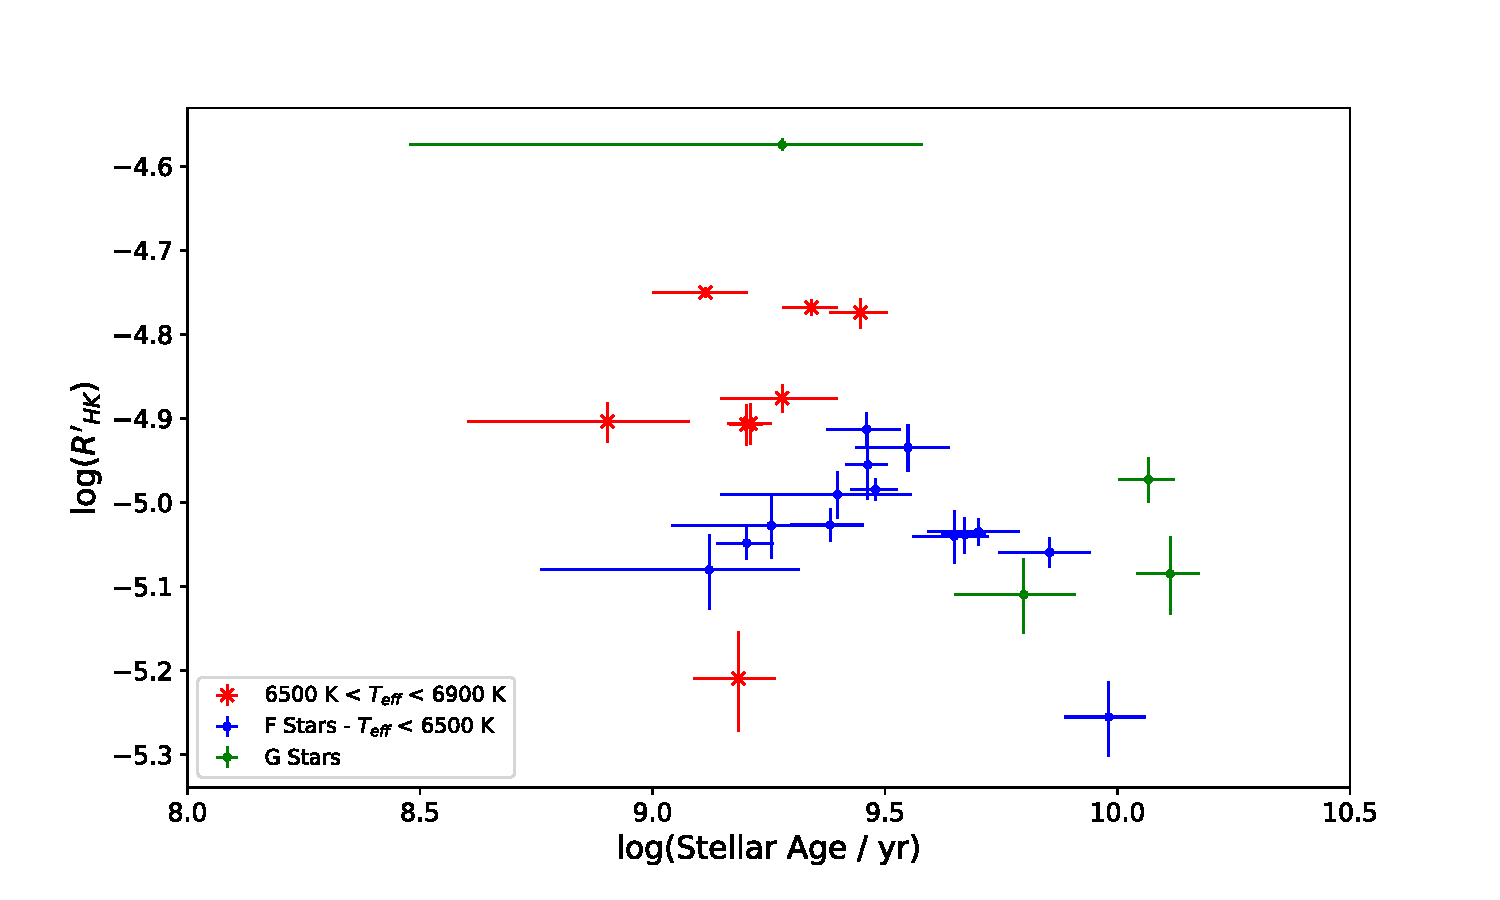
\includegraphics[scale=0.6]{Figures/4-Chromospheric_age/all_ca_results_h_order.pdf}
    \caption[Calcium age-activity plot using two channel analysis]{Plot showing the same sample as Figure \ref{fig:calcium_emission_plot}, but with \Rprime values calculated using only the H and R channels. This was in order to compare values with the archival observations found in the \esp archive at different epochs.}
    \label{fig:modified_ca_age_activity_plot_2channel}
\end{figure}

%App H
\chapter{\texorpdfstring{\Halpha}{Halpha} Results}
\label{App_halpha_results}
\begin{landscape}
\begin{longtable}{lccccccl}
\caption[Details of results from \Halpha analysis]{Results from \Halpha analysis. $B-V$ taken from SIMBAD \citep{Wenger_etal_2000}. Ages taken from asteroseismology studies \citep{Chaplin_etal_2014,Silva_Aguirre_etal_2017}.}\\

\hline
Star Name    & B-V  & $T_{eff}$ / K & $log(g)$ & Age / Gyr     & \Halpha Index & $log(I_{H\alpha})$         & Spectrograph   \\
\hline
\endfirsthead

\hline
Star Name    & B-V  & $T_{eff}$ / K & $log(g)$ & Age / Gyr     & \Halpha Index & $log(I_{H\alpha})$         & Spectrograph   \\
\hline
\endhead

\hline
\endfoot

\hline
\endlastfoot

KIC 1430163  & 0.49 & 6520 & 4.22   & $1.90^{0.60}_{0.50}$  & 0.0273        & $-1.460^{0.0020}$ & \narval        \\
KIC 1435467  & 0.43 & 6264 & 4.09   & $3.02^{0.35}_{0.35}$  & 0.0284        & $-1.445^{0.0010}$ & \narval        \\
KIC 2837475  & 0.45 & 6700 & 4.16   & $1.63^{0.18}_{0.18}$  & 0.0331        & $-1.392^{0.0015}$ & \esp           \\
KIC 3427720  & 0.55 & 6040 & 4.38   & $2.23^{0.24}_{0.24}$  & 0.0280        & $-1.454^{0.0016}$ & \esp           \\
KIC 3733735  & 0.43 & 6715 & 4.26   & $0.80^{0.40}_{0.40}$  & 0.0333        & $-1.390^{0.0018}$ & \esp           \\
KIC 4914923  & 0.60 & 5905 & 4.21   & $7.57^{1.79}_{1.79}$  & 0.0274        & $-1.465^{0.0016}$ & \esp           \\
KIC 5774694  & 0.64 & 5875 & 4.47   & $1.90^{1.90}_{1.60}$  & 0.0275        & $-1.468^{0.0016}$ & \esp           \\
KIC 5774694  & 0.64 & 5875 & 4.47   & $1.90^{1.90}_{1.60}$  & 0.0308        & $-1.428^{0.0011}$ & \narval        \\
KIC 6106415  & 0.55 & 5990 & 4.31   & $5.03^{1.12}_{1.12}$  & 0.0264        & $-1.474^{0.0012}$ & \narval        \\
KIC 6116048  & 0.59 & 5935 & 4.28   & $9.58^{1.90}_{1.90}$  & 0.0289        & $-1.446^{0.0020}$ & \esp           \\
KIC 6225718  & 0.50 & 6230 & 4.32   & $2.41^{0.43}_{0.43}$  & 0.0276        & $-1.456^{0.0016}$ & \narval        \\
KIC 6603624  & 0.78 & 5625 & 4.32   & $7.82^{0.86}_{0.86}$  & 0.0285        & $-1.475^{0.0018}$ & \esp           \\
KIC 7206837  & 0.46 & 6304 & 4.17   & $2.90^{0.30}_{0.30}$  & 0.0266        & $-1.468^{0.0018}$ & \narval        \\
KIC 7529180  & 0.42 & 6700 & 4.23   & $1.30^{0.30}_{0.30}$  & 0.0348        & $-1.375^{0.0015}$ & \narval        \\
KIC 7871531  & 0.66 & 5400 & 4.49   & $9.96^{1.77}_{1.77}$  & 0.0257        & $-1.494^{0.0015}$ & \esp           \\
KIC 7970740  & 0.74 & 5290 & 4.58   & $12.98^{2.00}_{2.00}$ & 0.0271        & $-1.487^{0.0018}$ & \esp           \\
KIC 8006161  & 0.85 & 5390 & 4.49   & $3.59^{1.45}_{1.45}$  & 0.0277        & $-1.497^{0.0017}$ & \esp           \\
KIC 8006161  & 0.85 & 5390 & 4.49   & $3.59^{1.45}_{1.45}$  & 0.0296        & $-1.472^{0.0041}$ & \narval        \\
KIC 8179536  & 0.50 & 6344 & 4.27   & $3.54^{0.81}_{0.81}$  & 0.0277        & $-1.455^{0.0011}$ & \narval        \\
KIC 8394589  & 0.55 & 6114 & 4.32   & $4.45^{0.83}_{0.83}$  & 0.0278        & $-1.456^{0.0010}$ & \narval        \\
KIC 8694723  & 0.46 & 6120 & 4.1    & $4.69^{0.51}_{0.51}$  & 0.0274        & $-1.458^{0.0016}$ & \narval        \\
KIC 8760414  & 0.52 & 5787 & 4.33   & $11.66^{1.61}_{1.61}$ & 0.0336        & $-1.388^{0.0017}$ & \narval        \\
KIC 9098294  & 0.57 & 5840 & 4.3    & $8.08^{0.73}_{0.73}$  & 0.0260        & $-1.481^{0.0023}$ & \narval        \\
KIC 9139151  & 0.51 & 6125 & 4.38   & $1.32^{0.75}_{0.75}$  & 0.0284        & $-1.447^{0.0014}$ & \esp           \\
KIC 9139163  & 0.48 & 6400 & 4.18   & $1.60^{0.22}_{0.22}$  & 0.0298        & $-1.429^{0.0021}$ & \esp           \\
KIC 9139163  & 0.48 & 6400 & 4.18   & $1.60^{0.22}_{0.22}$  & 0.0292        & $-1.436^{0.0009}$ & \narval        \\
KIC 9206432  & 0.44 & 6608 & 4.23   & $1.53^{0.30}_{0.30}$  & 0.0254        & $-1.483^{0.0018}$ & \esp           \\
KIC 9226926  & 0.41 & 6892 & 4.14   & $2.20^{0.30}_{0.30}$  & 0.0277        & $-1.455^{0.0018}$ & \narval        \\
KIC 9955598  & 0.72 & 5410 & 4.48   & $6.29^{1.84}_{1.84}$  & 0.0282        & $-1.469^{0.0017}$ & \narval        \\
KIC 10016239 & 0.54 & 6340 & 4.31   & $1.80^{0.80}_{0.70}$  & 0.0299        & $-1.430^{0.0011}$ & \narval        \\
KIC 10454113 & 0.52 & 6120 & 4.31   & $2.89^{0.53}_{0.53}$  & 0.0316        & $-1.410^{0.0019}$ & \esp           \\
KIC 10454113 & 0.52 & 6120 & 4.31   & $2.89^{0.53}_{0.53}$  & 0.0287        & $-1.443^{0.0015}$ & \narval        \\
KIC 10462940 & 0.56 & 6154 & 4.32   & $2.50^{1.10}_{1.10}$  & 0.0280        & $-1.455^{0.0013}$ & \narval        \\
KIC 10644253 & 0.59 & 6030 & 4.4    & $2.39^{0.96}_{0.96}$  & 0.0281        & $-1.456^{0.0014}$ & \esp           \\
KIC 10709834 & 0.44 & 6508 & 4.09   & $2.80^{0.40}_{0.40}$  & 0.0270        & $-1.463^{0.0011}$ & \narval        \\
KIC 10963065 & 0.51 & 6060 & 4.29   & $7.15^{1.61}_{1.61}$  & 0.0296        & $-1.433^{0.0017}$ & \narval        \\
KIC 11081729 & 0.42 & 6630 & 4.25   & $1.88^{0.42}_{0.42}$  & 0.0268        & $-1.465^{0.0016}$ & \esp           \\
KIC 11253226 & 0.39 & 6605 & 4.16   & $1.60^{0.13}_{0.13}$  & 0.0310        & $-1.417^{0.0015}$ & \esp           \\
KIC 12009504 & 0.55 & 6065 & 4.21   & $3.97^{0.43}_{0.43}$  & 0.0342        & $-1.384^{0.0013}$ & \esp           \\
\end{longtable}
\clearpage
\end{landscape}


%Appendix I
\chapter{Rotation-activity data}
\label{App_I_activity_rotation}

\begin{landscape}
\begin{longtable}{llccccccl}

\caption[Details of activity and rotation parameters for sample of stars]{\begin{footnotesize} 	Activity and rotation indicator values for sample of stars considered for the activity-rotation analysis. References indicate the sources for the rotation period, chromospheric emission and X-ray emission, respectively. Note that $nan$ errors denote where literature values do not provide error bars.
\noindent
\textbf{References}: (1) \citet{Davies_etal_2015}; (2) \citet{Boro_Saikia_etal_2016}; (3) \citet{Vaughan_etal_1981}; (4) \citet{DeWarf_etal_2010}; (5) \citet{Robertson_etal_2015_GJ176}; (6) \citet{Robertson_etal_2015_GJ191}; (7) \citet{Ammler_vonEiff_Reiners_2012}; (8) \citet{McQuillan_etal_2014} - * indicates low significance for $P_{rot}$; (9) \citet{Paz_Chinchon_etal_2015}; (10) \citet{Nielsen_etal_2013}; (11) \citet{Garcia_etal_2014}; (12) \citet{Janes_2017}; (13) \citet{Collins_etal_2017}; (14) Average \Rprime values from \citet{Pace_2013}; (15) \citet{Sissa_etal_2016}; (16) \citet{Mamajek_Hillenbrand_2008}; (17) \citet{Astudillo_Defru_etal_2017}; (18) \citet{Murgas_etal_2013}; (19) Calcium Study presented in Chapter \ref{Chapter4}; (20) \citet{Egeland_etal_2017}; (21) \citet{Booth_etal_2017}
\end{footnotesize}}\\

\hline
Star Name    & $P_{rot}$ / days        & $log(R^{'}_{HK})$ & log($L_{x}/R_{\odot}^{2}$ / ergs s$^{-1}$ $R_{\odot}^{-2}$)          & References& \tauc   & \Ro \\
\hline
\endfirsthead

\hline
Star Name    & $P_{rot}$ / days        & $log(R^{'}_{HK})$ & log($L_{x}/R_{\odot}^{2}$ / ergs s$^{-1}$ $R_{\odot}^{-2}$)          & References& \tauc   & \Ro \\
\hline
\endhead

\hline
\endfoot

\hline
\endlastfoot

16 Cyg A     & $23.80^{1.80}$   & $-4.909^{0.2}$    & $26.71^{0.10}$    & 1,14,21       & 13.45  & $1.77_{0.18}^{0.19}$  \\
16 Cyg B     & $23.20^{5.00}$   & $-4.935^{0.119}$  & $<25.77$          & 1,14,21       & 14.71  & $1.58_{0.38}^{0.40}$  \\
61 Cyg A     & $35.70^{1.90}$   & $-4.850^{0.106}$  & $27.43^{0.10}$    & 2,14,21       & 24.33  & $1.47_{0.08}^{0.08}$  \\
61 Cyg B     & $48.00^{0.5}$    & $-4.950^{nan}$    & $27.33^{0.23}$    & 3,15,21       & 28.80  & $1.67_{nan}^{nan}$    \\
Alpha Cen B  & $36.20^{1.40}$   & $-4.920^{nan}$    & $27.19^{0.36}$    & 4,16,21       & 15.98  & $2.26_{0.11}^{0.11}$  \\
GJ 176       & $39.46^{0.01}$   & $-4.911^{nan}$    & $27.8^{0.10}$     & 5,17,21       & 36.27  & $1.09_{0.08}^{0.08}$  \\
GJ 191       & $142.90^{0.30}$  & $-4.774^{nan}$    & $27.02^{0.10}$    & 6,17,21       & 68.02  & $2.10_{0.20}^{0.21}$  \\
HR 7703      & $17.10^{0.5}$    & $-4.929^{nan}$    & $27.04^{0.10}$    & 7,18,21       & 21.15  & $0.81_{0.08}^{0.09}$  \\
KIC 10016239 & $4.89^{0.03}$    & $-5.090^{0.063}$  & $27.71^{0.10}$    & 8,19,21       & 11.25  & $0.43_{0.03}^{0.03}$  \\
KIC 10454113 & $14.45^{0.23}$   & $-4.903^{0.027}$  & N/A               & 8,19,N/A      & 11.39  & $1.27_{0.07}^{0.07}$  \\
KIC 10963065 & $12.96^{0.05}$   & $-5.089^{0.025}$  & N/A               & 9,19,N/A      & 14.71  & $0.88_{0.08}^{0.09}$  \\
KIC 12011630 & $45.03^{7.59}$   & N/A               & $<30.05$          & 8*,N/A,21     & 16.39  & $2.75_{0.60}^{0.67}$  \\
KIC 1435467  & $6.96^{0.39}$    & $-5.033^{0.018}$  & N/A               & 10,19,N/A     & 9.40   & $0.74_{0.08}^{0.09}$  \\
KIC 3123191  & $20.55^{0.09}$   & N/A               & $<28.84$          & 8,N/A,21      & 11.87  & $1.73_{0.12}^{0.13}$  \\
KIC 3733735  & $2.57^{0.01}$    & $-4.983^{0.045}$  & N/A               & 8,19,N/A      & 8.63   & $0.30_{0.02}^{0.02}$  \\
KIC 5309966  & $10.97^{0.91}$   & N/A               & $<29.02$          & 11,N/A,21     & 9.88   & $1.11_{0.14}^{0.15}$  \\
KIC 6116048  & $17.26^{1.96}$   & N/A               & $<26.74$          & 11,N/A,21     & 15.86  & $1.09_{0.20}^{0.22}$  \\
KIC 6225718  & $7.32^{1.20}$    & $-5.111^{0.032}$  & N/A               & 12,19,N/A     & 11.54  & $0.63_{0.13}^{0.13}$  \\
KIC 6603624  & $45.32^{2.16}$   & N/A               & $<26.96$          & 8*,N/A,21     & 14.26  & $3.18_{0.28}^{0.29}$  \\
KIC 7206837  & $4.07^{0.01}$    & $-4.987^{0.062}$  & N/A               & 8,19,N/A      & 9.64   & $0.42_{0.02}^{0.02}$  \\
KIC 7529180  & $1.92^{0.36}$    & N/A               & $28.66^{0.10}$    & 11,N/A,21     & 9.76   & $0.20_{0.04}^{0.05}$  \\
KIC 8179536  & $25.65^{0.53}$   & $-4.937^{0.039}$  & N/A               & 10,19,N/A     & 11.54  & $2.22_{0.22}^{0.24}$  \\
KIC 9025370  & $24.51^{2.56}$   & N/A               & $<27.23$          & 8*,N/A,21     & 15.14  & $1.62_{0.24}^{0.25}$  \\
KIC 9139151  & $12.22^{0.70}$   & $-5.061^{0.074}$  & N/A               & 12,19,N/A     & 11.25  & $1.09_{0.13}^{0.14}$  \\
KIC 9139163  & $0.61^{0.01}$    & $-5.095^{0.027}$  & N/A               & 12,19,N/A     & 8.54   & $0.07_{0}^{0}$        \\
KIC 9410862  & $22.77^{2.37}$   & N/A               & $<27.86$          & 11,N/A,21     & 15.14  & $1.50_{0.26}^{0.28}$  \\
KIC 9955598  & $34.20^{5.64}$   & $-4.934^{0.046}$  & $27.01^{0.10}$    & 11,19,21      & 16.89  & $2.02_{0.44}^{0.49}$  \\
Proxima Cen  & $82.60^{1.00}$   & $-5.003^{nan}$    & $28.23^{0.10}$    & 13,17,21      & 118.62 & $0.70_{0.04}^{0.04}$  \\
Sun          & $27.00^{3.00}$   & $-4.943^{0.042}$  & $26.77^{0.72}$    & N/A,20,21     & 14.45  & $1.87_{0.21}^{0.21}$  \\

\end{longtable}
\clearpage
\end{landscape}




\end{appendices}